\documentclass{beamer}

\usetheme{Madrid}
\usecolortheme{default}
\usefonttheme{professionalfonts}
\useinnertheme{rounded}

% --- PREÁMBULO ---
\usepackage[utf8]{inputenc}
\usepackage[T1]{fontenc}
\usepackage[spanish]{babel}
\usepackage{amsmath, amssymb}
\usepackage{graphicx}
\usepackage{tikz}
\usetikzlibrary{positioning, calc, arrows.meta}
\usepackage{pgfplots}
\pgfplotsset{compat=1.18}
\usepackage{tcolorbox}
\usepackage{ragged2e}
\usepackage{array}
\usepackage{booktabs}
\usetikzlibrary{shapes, arrows, positioning, calc}
      % Para mejorar control de columnas en tablas
\usepackage{multicol}        % Para usar múltiples columnas de forma más flexible

\usetikzlibrary{arrows.meta, positioning, shapes.geometric, calc, fit}
\usepackage{caption} % Para usar \captionof
\usepackage{media9}
\usepackage{listings}
\usepackage{xcolor}
\usepackage{hyperref}





\newcommand{\figplaceholder}[2][0.6\textwidth]{%
    \begin{tikzpicture}
        \node[draw, dashed,
              minimum width=#1,       % Ancho total del cuadro del nodo
              text width=0.9*#1,      % Ancho para el texto dentro del nodo (90% del ancho total)
              minimum height=0.5*#1,  % Alto del nodo (50% del ancho total)
              align=center,           % Alineación del texto
              text=gray,              % Color del texto
              inner sep=3pt           % Espacio interno alrededor del texto
              ] {#2};
    \end{tikzpicture}%
}


% --- METADATOS DE LA PRESENTACIÓN ---
\title{Transformaciones de Intensidad y Filtrado Espacial}
\subtitle{Basado en el Cap. 3 de "Digital Image Processing" \\ (Gonzalez \& Woods)}
\author{Nombre del Presentador  \small{(Adaptado de material técnico)}}
\institute{Universidad / Institución}
\date{\today}

\begin{document}

% --- DIAPOSITIVA DE TÍTULO ---
\begin{frame}
    \titlepage
\end{frame}
%%% --- FIN DE DIAPOSITIVA --- %%%

% --- DIAPOSITIVA DE CONTENIDO (TABLA DE MATERIAS) ---
\begin{frame}
    \frametitle{Contenido}
    \tableofcontents
\end{frame}
%%% --- FIN DE DIAPOSITIVA --- %%%

% --- SECCIÓN 1 ---
\section{Introducción y Conceptos Fundamentales}

\begin{frame}{Preview del Capítulo}
    \begin{block}{Dominio Espacial}
        El término \textit{dominio espacial} se refiere al plano mismo de la imagen, y los métodos de procesamiento en esta categoría se basan en la manipulación directa de los píxeles en una imagen.
    \end{block}
    \begin{itemize}
        \item Se contrasta con el procesamiento en el \textit{dominio de la frecuencia} (o transformado), donde la imagen primero se transforma, luego se procesa, y finalmente se aplica la transformada inversa.
        \item Dos categorías principales de procesamiento en el dominio espacial:
        \begin{itemize}
            \item \textbf{Transformaciones de intensidad}: Operan en píxeles individuales. Útiles para manipulación de contraste y segmentación por umbralización.
            \item \textbf{Filtrado espacial}: Realiza operaciones sobre la vecindad de cada píxel. Útil para suavizado y realce de bordes.
        \end{itemize}
    \end{itemize}
\end{frame}
%%% --- FIN DE DIAPOSITIVA --- %%%

\begin{frame}{Objetivos de Aprendizaje}
    Al finalizar este capítulo, el lector debería ser capaz de:
    \begin{columns}[T,onlytextwidth]
        \begin{column}{0.5\textwidth}
            \begin{itemize}
                \item Entender el significado del procesamiento en el dominio espacial y cómo difiere del procesamiento en el dominio de la frecuencia.
                \item Conocer las técnicas principales utilizadas para las transformaciones de intensidad.
                \item Comprender el significado físico de los histogramas de imagen y cómo pueden ser manipulados para el realce.
                \item Entender la mecánica del filtrado espacial y cómo se forman los filtros espaciales.
            \end{itemize}
        \end{column}
        \begin{column}{0.5\textwidth}
            \begin{itemize}
                \item Entender los principios de la convolución y correlación espacial.
                \item Familiarizarse con los principales tipos de filtros espaciales y cómo se aplican.
                \item Ser consciente de las relaciones entre los filtros espaciales y el concepto fundamental de los filtros paso bajo.
                \item Entender cómo se pueden utilizar combinaciones de métodos de realce cuando un solo enfoque es insuficiente.
            \end{itemize}
        \end{column}
    \end{columns}
\end{frame}
%%% --- FIN DE DIAPOSITIVA --- %%%

% --- SECCIÓN 2 ---
\section{Principios Básicos de Transformaciones de Intensidad y Filtrado Espacial}

\begin{frame}{Procesos en el Dominio Espacial}
    \begin{block}{Definición General}
    Los procesos en el dominio espacial se expresan comúnmente como:
    \begin{equation}\label{eq:general_transform_final}
        g(x, y) = T[f(x, y)]
    \end{equation}
    donde:
    \begin{itemize}
        \item $f(x, y)$ es la imagen de entrada.
        \item $g(x, y)$ es la imagen procesada (salida).
        \item $T$ es un operador definido sobre una vecindad del punto $(x, y)$.
    \end{itemize}
    El punto $(x_0, y_0)$ es una ubicación arbitraria en la imagen, y la región pequeña alrededor de este es su \textit{vecindad}.
    \end{block}
\end{frame}
%%% --- FIN DE DIAPOSITIVA --- %%%

\begin{frame}{Vecindad de un píxel}
    \centering % Centra la imagen sin el entorno figure
    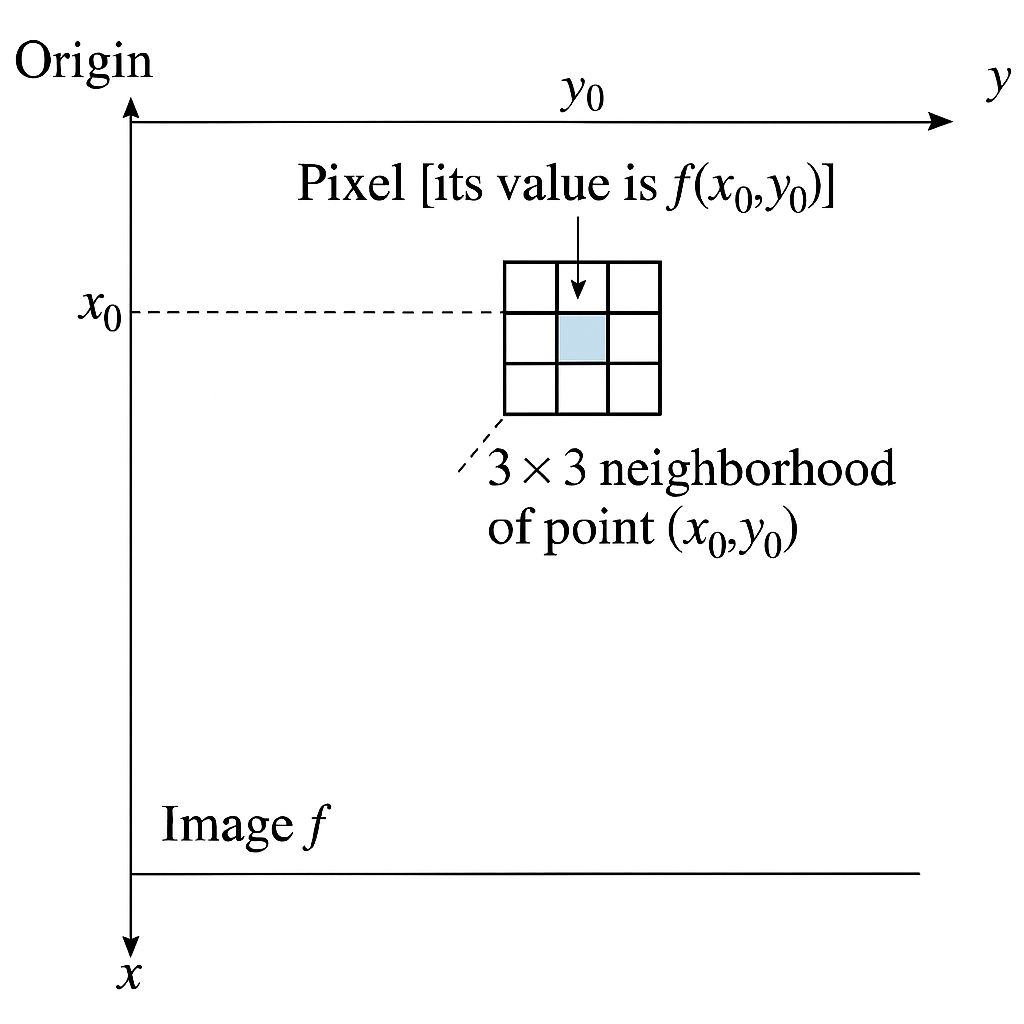
\includegraphics[width=0.7\linewidth]{figuras/Fig_3_1.png}
    \captionof{figure}{Representación de una vecindad $3 \times 3$ centrada en $(x_0, y_0)$.} % Usar \captionof
\end{frame}
%\begin{frame}{Vecindad de un píxel}
%    \begin{figure}
%        \centering
%        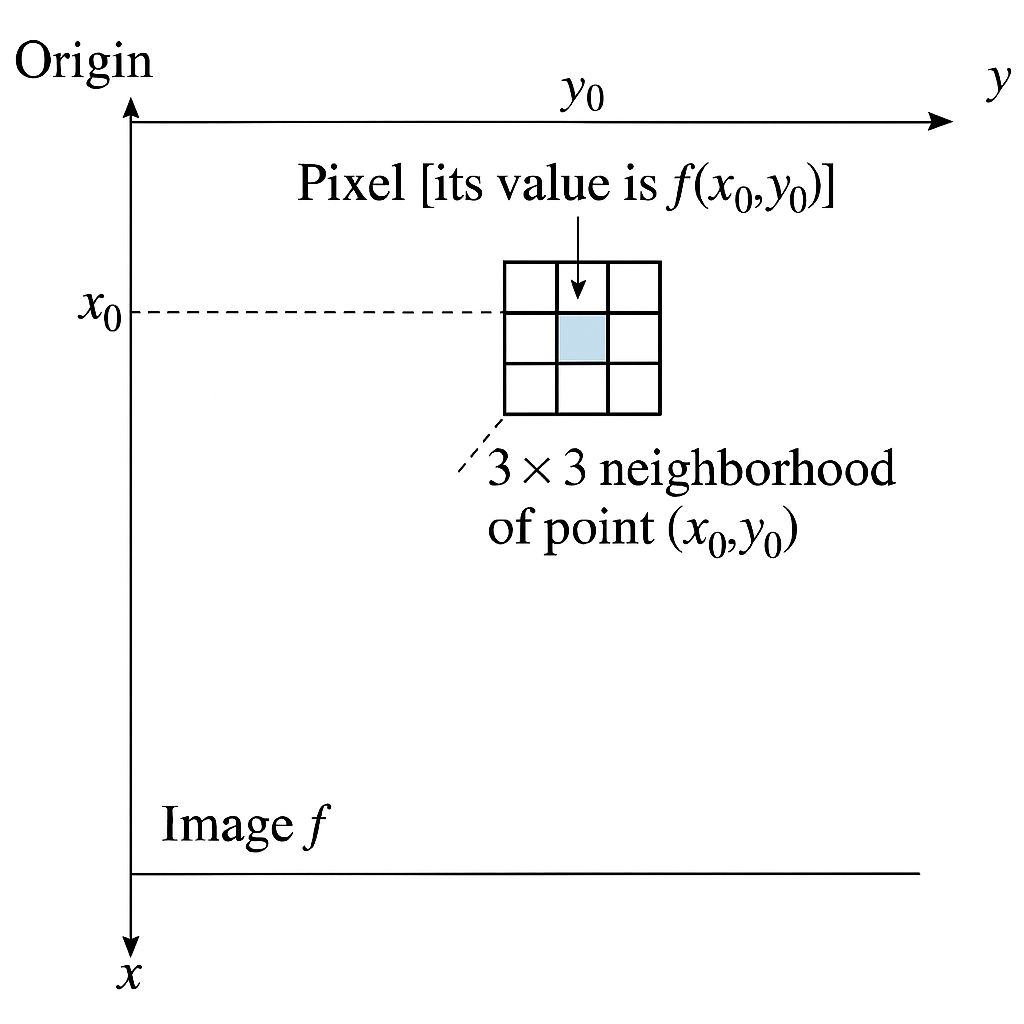
\includegraphics[width=0.7\linewidth]{figuras/Fig_3_1.png}
%        \caption{Representación de una vecindad $3 \times 3$ centrada en $(x_0, y_0)$.}
%    \end{figure}
%\end{frame}


\begin{frame}{Operador $T$ y Vecindad (Neighborhood)}
    \begin{block}{Ilustración de la Vecindad (Original: Fig. 3.1)}
        Una vecindad de $3 \times 3$ alrededor de un punto $(x_0, y_0)$ en una imagen $f$. La vecindad se mueve de píxel a píxel en la imagen para generar una imagen de salida. El valor del píxel en $(x_0, y_0)$ es $f(x_0, y_0)$.
    \end{block}
    \begin{figure}
        \centering
        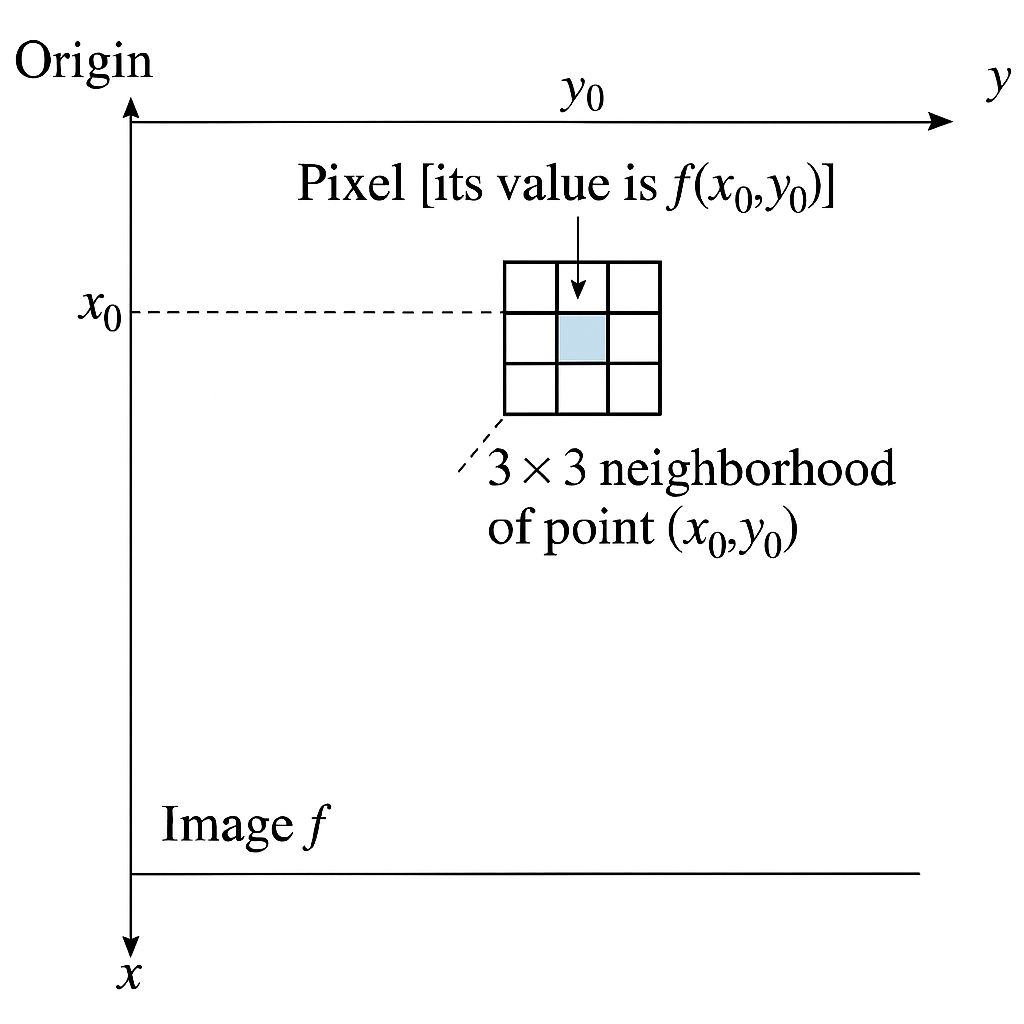
\includegraphics[width=0.4\linewidth]{figuras/Fig_3_1.png}
        \caption{Representación de una vecindad $3 \times 3$ centrada en $(x_0, y_0)$.}
    \end{figure}
\end{frame}
%%% --- FIN DE DIAPOSITIVA --- %%%

\begin{frame}{Transformaciones de Intensidad (Mapeo de Nivel de Gris)}
    \begin{block}{Definición}
    La forma más simple del operador $T$ es cuando la vecindad es de tamaño $1 \times 1$. En este caso, el valor de salida $g$ en $(x,y)$ solo depende del valor de $f$ en ese mismo punto. Esto se conoce como una \textbf{transformación de nivel de gris} o \textbf{función de mapeo de intensidad}, y se denota como:
    \begin{equation}\label{eq:intensity_transform_final}
        s = T(r)
    \end{equation}
    donde:
    \begin{itemize}
        \item $r$ denota el nivel de gris (intensidad de entrada) de $f(x,y)$.
        \item $s$ denota el nivel de gris (intensidad de salida) de $g(x,y)$.
    \end{itemize}
    \end{block}
    \begin{exampleblock}{Ejemplos Comunes de $T(r)$}
        \begin{itemize}
            \item \textbf{Estiramiento de contraste (Contrast stretching)}: Para expandir el rango dinámico de los niveles de gris.
            \item \textbf{Umbralización (Thresholding)}: Para crear una imagen binaria. Si $T(r)$ es una función escalón, se llama función de umbralización.
        \end{itemize}
    \end{exampleblock}
\end{frame}
%%% --- FIN DE DIAPOSITIVA --- %%%

\begin{frame}{Ejemplos Gráficos de $T(r)$ (Fig. 3.2 Mejorada)}
    \begin{figure}
        \centering
        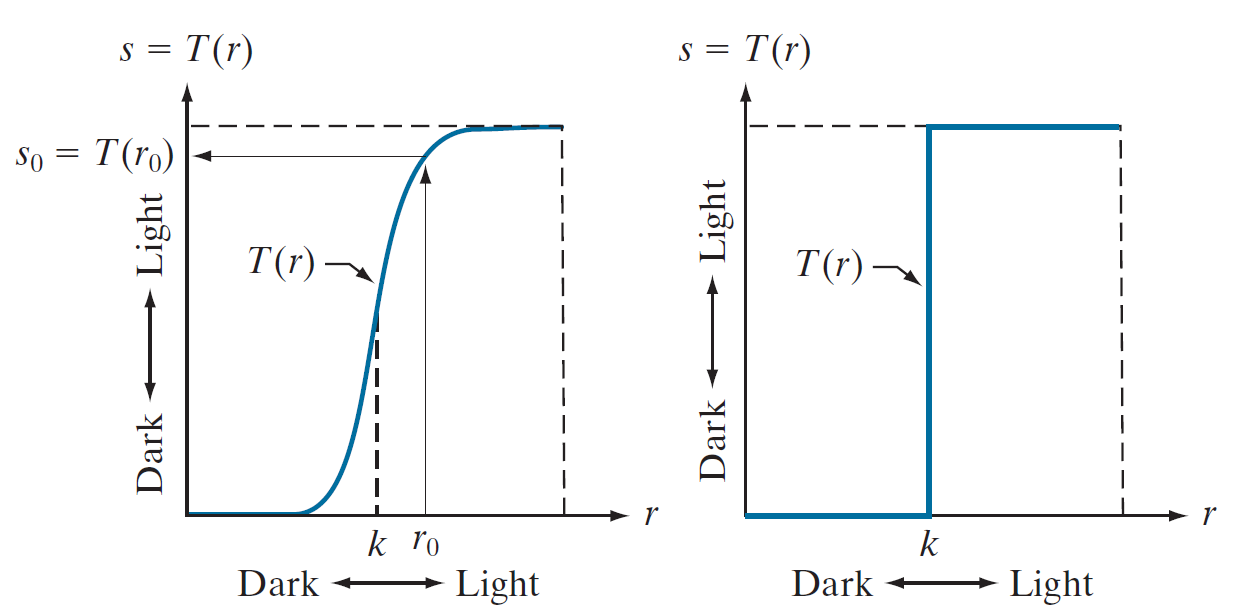
\includegraphics[width=0.8\linewidth]{figuras/Fig_3_2.png}
        \caption{3.2}
    \end{figure}
\end{frame}
%%% --- FIN DE DIAPOSITIVA --- %%%

% --- SECCIÓN 3 ---
\section{Acerca de los Ejemplos en este Capítulo}

\begin{frame}\footnotesize{{Relevancia de los Ejemplos}
    \begin{alertblock}{Enfoque Principal: Realce de Imágenes}
        Aunque las transformaciones de intensidad y el filtrado espacial abarcan una amplia gama de aplicaciones, la mayoría de los ejemplos en este capítulo se centran en aplicaciones para el \textbf{realce de imágenes}.
    \end{alertblock}
    \begin{itemize}
        \item \textbf{Realce}: Proceso de manipular una imagen para que el resultado sea más adecuado que el original para una aplicación específica.
        \item La palabra específica es crucial: lo que funciona para realzar imágenes de rayos X puede no ser óptimo para imágenes infrarrojas.
        \item No existe una "teoría" general del realce de imágenes. Cuando se procesan imágenes para interpretación visual, el observador es el juez final de cuán bien funciona un método particular.
        \item El realce para percepción automática (machine perception) es más fácil de cuantificar.
    \end{itemize}
    \begin{exampleblock}{Propósito Ilustrativo}
    El uso de ejemplos de realce de imágenes sirve como una forma efectiva de introducir las técnicas de procesamiento espacial. El material desarrollado tiene un alcance mucho más amplio que solo el realce de imágenes.
    \end{exampleblock}}
\end{frame}
%%% --- FIN DE DIAPOSITIVA --- %%%

% --- DIAPOSITIVA DE RESUMEN (EJEMPLO) ---
\begin{frame}
    \frametitle{Resumen y Puntos Clave}
    \begin{itemize}
        \item Las \textbf{transformaciones de intensidad} operan a nivel de píxel individual, modificando su valor basándose en una función $s=T(r)$.
        \item El \textbf{filtrado espacial} opera sobre una vecindad de píxeles para calcular el valor de salida del píxel central de dicha vecindad.
        \item Ambas son técnicas fundamentales en el dominio espacial para el preprocesamiento y realce de imágenes.
        \item Ecuaciones fundamentales:
        \begin{itemize}
            \item Transformación general en el dominio espacial: \(g(x, y) = T[f(x, y)]\)
            \item Transformación de intensidad (mapeo de nivel de gris): \(s = T(r)\)
        \end{itemize}
    \end{itemize}
    \begin{block}{Próximos Pasos en el Estudio}
        La discusión continuará con el procesamiento de histogramas, diferentes tipos de filtros espaciales (suavizado, realce) y sus aplicaciones detalladas.
    \end{block}
\end{frame}

%%%%%%%%%%%%%%%%%%%%%%%%%%%%%%%%%%%%%%%%%%%%%%%%%%%%%%%%%%%%%%%%%%%%%%%%%%%%%%%%%%%%%%%%%%%%%%%%%%%%%%%%%%%%%%%%%%%%%%%%%%%%%%%%%%%%%%%%%%%%%%%%%%%%%%%%%%%%%%%%%%


% --- Título ---
\title{Transformaciones Básicas de Intensidad en Imágenes Digitales}
\author{Procesamiento Digital de Imágenes}
\institute{Basado en literatura académica de referencia}
\date{}

% --- Diapositiva de título ---
\begin{frame}
  \titlepage
\end{frame}

% --- Introducción ---
\begin{frame}{Funciones de Transformación de Intensidad}
\begin{block}{Definición}
Las transformaciones de intensidad modifican los niveles de gris de una imagen, mapeando cada valor de entrada \( r \) a una salida \( s = T(r) \).
\end{block}
\vspace{1em}
\begin{itemize}
    \item Son implementadas por tablas de búsqueda (LUTs).
    \item Para una imagen de 8 bits: 256 posibles valores.
    \item Se agrupan en funciones: lineales, logarítmicas y de potencia.
\end{itemize}
\end{frame}

% --- Tipos de transformaciones ---
\begin{frame}{Tipos de Transformaciones}
\begin{block}{Clasificación}
\begin{itemize}
    \item \textbf{Lineales:} Transformación negativa e identidad.
    \item \textbf{Logarítmicas:} Logarítmica e inversa logarítmica.
    \item \textbf{Potencia:} \( n \)-ésima potencia y raíz \( n \)-ésima.
\end{itemize}
\end{block}
\end{frame}

% --- Ecuación imagen negativa ---
\begin{frame}{Transformación Negativa}
\begin{block}{Ecuación}
Para una imagen con niveles de intensidad en el rango \( [0, L-1] \), su negativo se define como:
\[
s = L - 1 - r \tag{3-3}
\]
\end{block}
\pause
\begin{alertblock}{Aplicaciones}
\begin{itemize}
    \item Realce de detalles en áreas oscuras.
    \item Utilidad clínica: imágenes médicas (mamografías).
\end{itemize}
\end{alertblock}
\end{frame}

% --- Figura TikZ corregida ---
\begin{frame}{Curvas de Transformación de Intensidad}
\begin{figure}
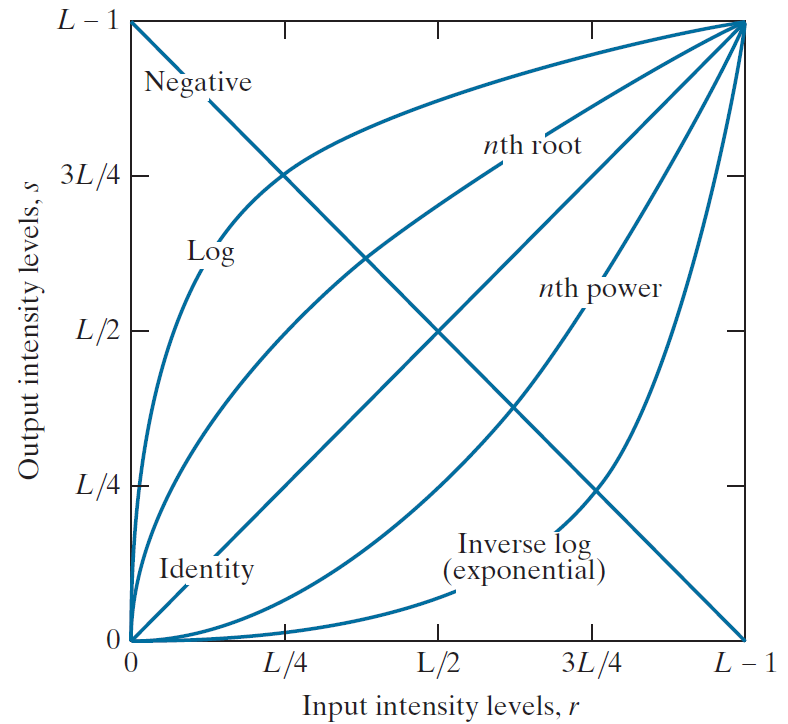
\includegraphics[width=0.5\linewidth]{figuras/Fig_3_3.png}
\caption{Tipos de funciones de transformación de intensidad.}
\end{figure}
\end{frame}

% --- Imágenes médicas ---
\begin{frame}{Ejemplo Clínico: Mamografía}
\centering
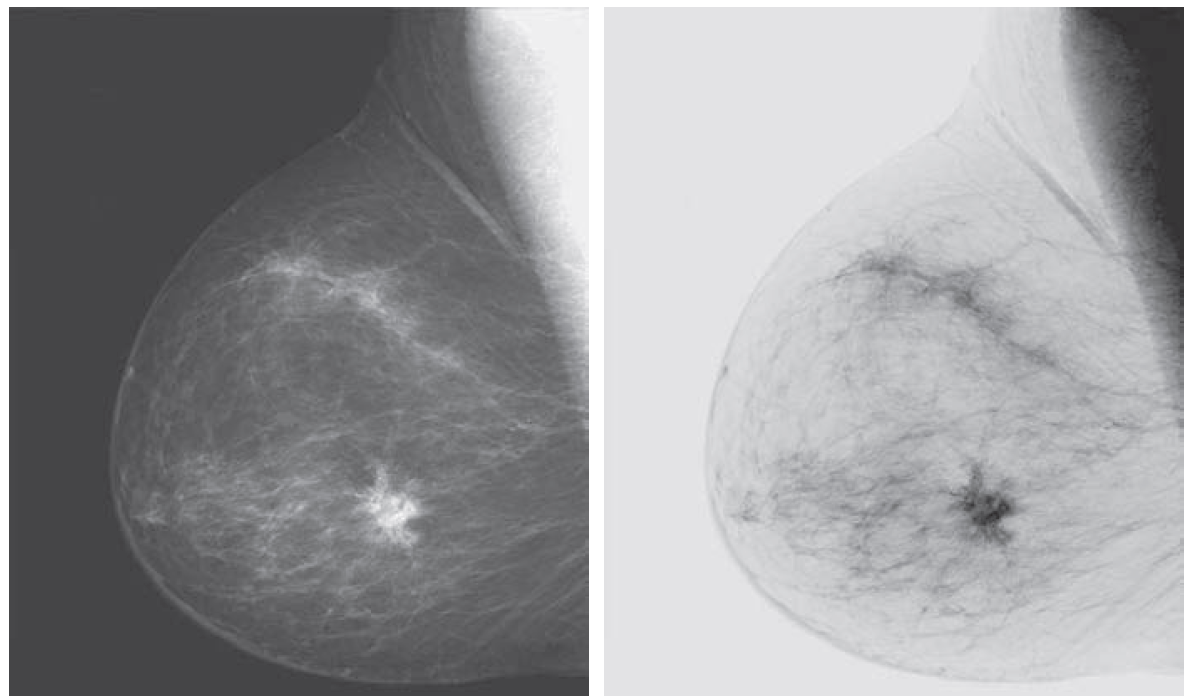
\includegraphics[width=0.6\linewidth]{figuras/Fig_3_4.png}
\begin{block}{Observación}
El negativo puede facilitar el análisis de detalles en tejidos blandos como el tejido mamario.
\end{block}
\end{frame}

% --- Resumen ---
\begin{frame}{Resumen}
\begin{itemize}
    \item Las transformaciones de intensidad son herramientas fundamentales para mejorar imágenes.
    \item Incluyen funciones lineales, logarítmicas y de potencia.
    \item La transformación negativa es útil en contextos clínicos y de contraste inverso.
\end{itemize}
\end{frame}

%%%%%%%%%%%%%%%%%%%%%%%%%%%%%%%%%%%%%%%%%%%%%%%%%%%%%%%%%%%%%%%%%%%%%%%%%%%%%%%%%%%%%%%%%%%%%%%%%%%%%%%%%%%%%%%%%

% --- Titulo ---
\title{Transformaciones Logar\'itmicas y de Potencia (Gamma)}
\author{Procesamiento Digital de Im\'agenes}
\institute{Basado en literatura acad\'emica de referencia}
\date{}

% --- Diapositiva de título ---
\begin{frame}
  \titlepage
\end{frame}

% === TRANSFORMACIÓN LOGARÍTMICA ===
\begin{frame}{Transformación Logar\'itmica}
\begin{block}{Ecuaci\'on}
\[
s = c \log(1 + r) \tag{3-4}
\]
\end{block}
\begin{itemize}
    \item Expande intensidades bajas, comprime altas.
    \item Aplicada a espectros (por ejemplo, Fourier).
    \item Mejora visualizaci\'on de detalles sutiles.
\end{itemize}
\end{frame}

\begin{frame}{Ejemplo Espectro de Fourier}
\begin{figure}
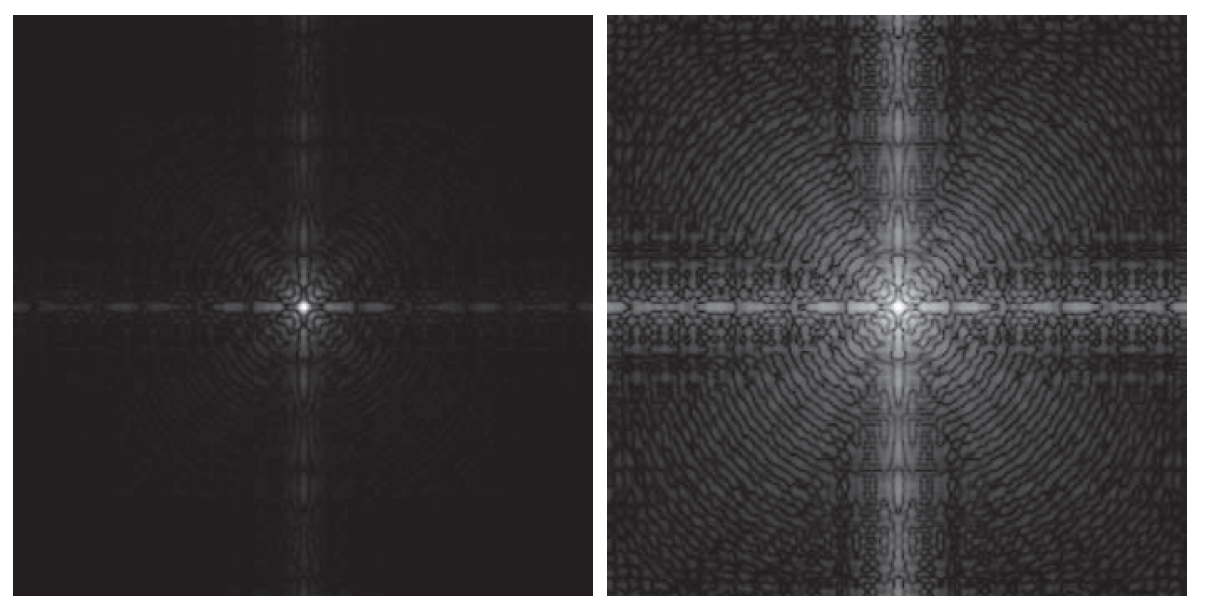
\includegraphics[width=0.8\linewidth]{figuras/Fig_3_5.png}
\caption{(a) Fourier spectrum displayed as a grayscale image. (b) Result of applying the log transformation in Eq. (3-4) with c = 1. Both images are scaled to the range [0, 255].}
\end{figure}
\end{frame}

% === TRANSFORMACIÓN POTENCIA ===
\begin{frame}{Transformaci\'on Potencia (Gamma)}
\begin{block}{Ecuaci\'on}
\[
s = c r^\gamma \tag{3-5}
\]
\end{block}
\begin{itemize}
    \item Control de brillo y contraste.
    \item \textbf{Correcci\'on gamma} para pantallas.
    \item Cuando \( \gamma = 1 \), se obtiene la identidad.
\end{itemize}
\end{frame}

\begin{frame}{Curvas Gamma (Fig. 3.6)}
\centering
\begin{figure}
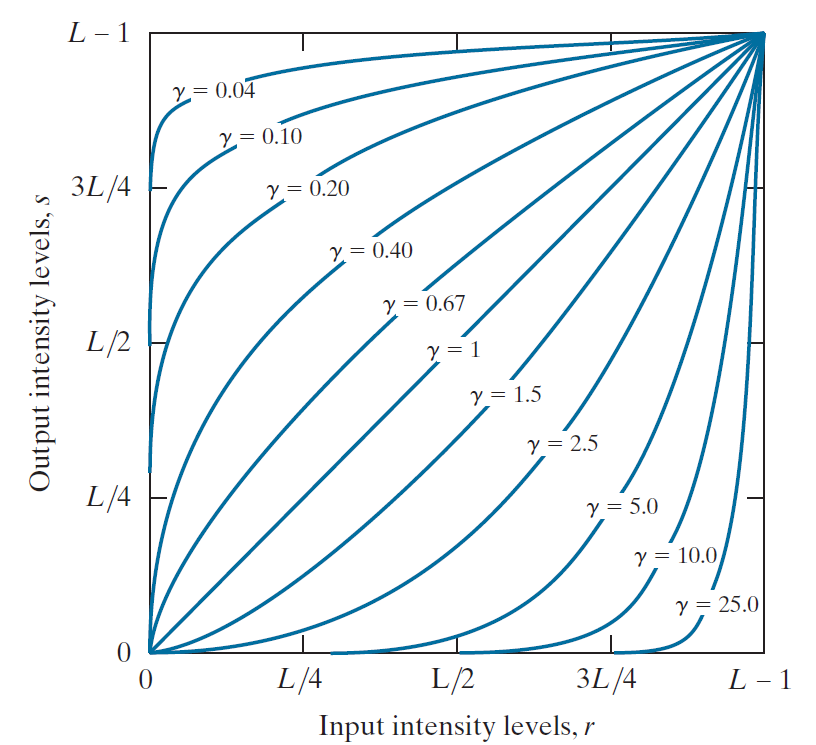
\includegraphics[width=0.5\linewidth]{figuras/Fig_3_6.png}
\caption{\footnotesize{Plots of the gamma equation
s = c rg for various
values of g (c = 1
in all cases). Each
curve was scaled
independently so
that all curves
would fit in the
same graph. Our
interest here is
on the shapes of
the curves, not
on their relative
values.}}
\end{figure}
\end{frame}

\begin{frame}{Simulaci\'on y Correcci\'on Gamma (Fig. 3.7)}
\centering
\begin{figure}
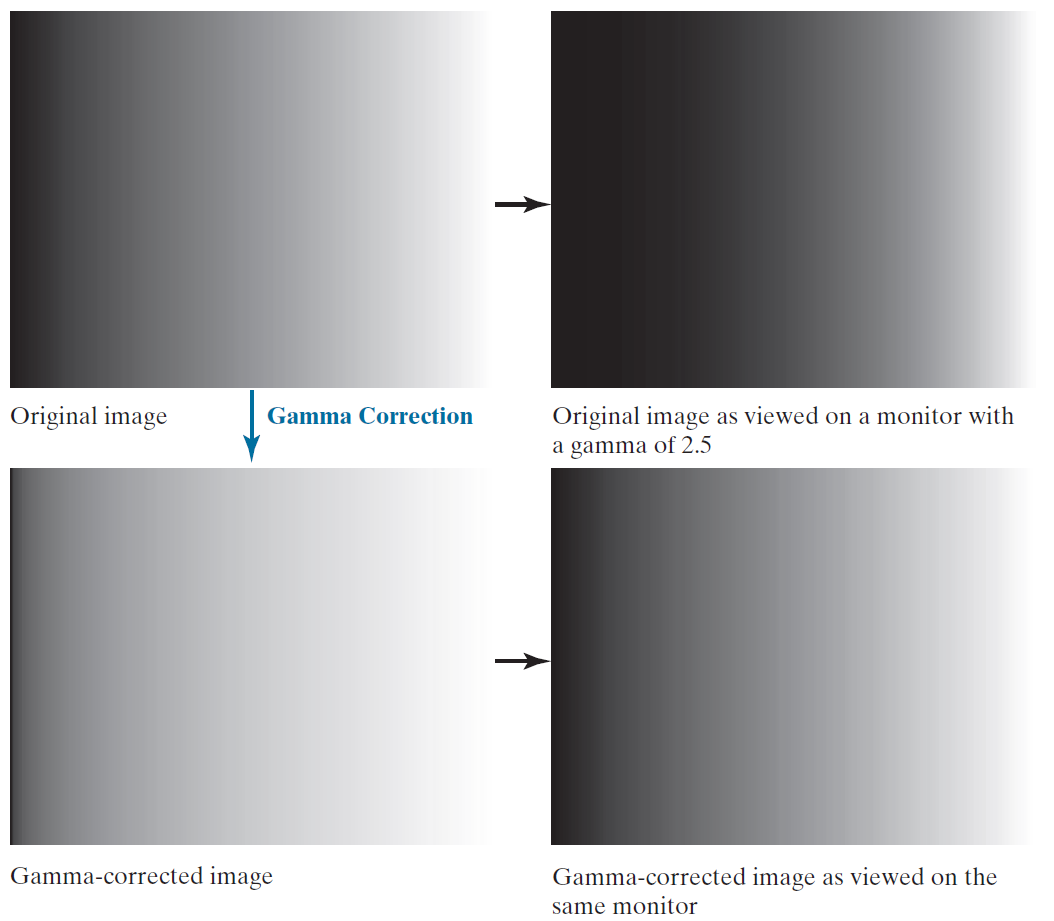
\includegraphics[width=0.6\linewidth]{figuras/Fig_3_7.png}
\caption{\footnotesize{(a) Intensity ramp
image. (b) Image
as viewed on a
simulated monitor
with a gamma of
2.5. (c) Gammacorrected
image.
(d) Corrected
image as viewed
on the same
monitor. Compare
(d) and (a).}}
\end{figure}
\end{frame}

\begin{frame}{Aplicaci\'on Cl\'inica: MRI (Fig. 3.8)}
\centering
\begin{figure}
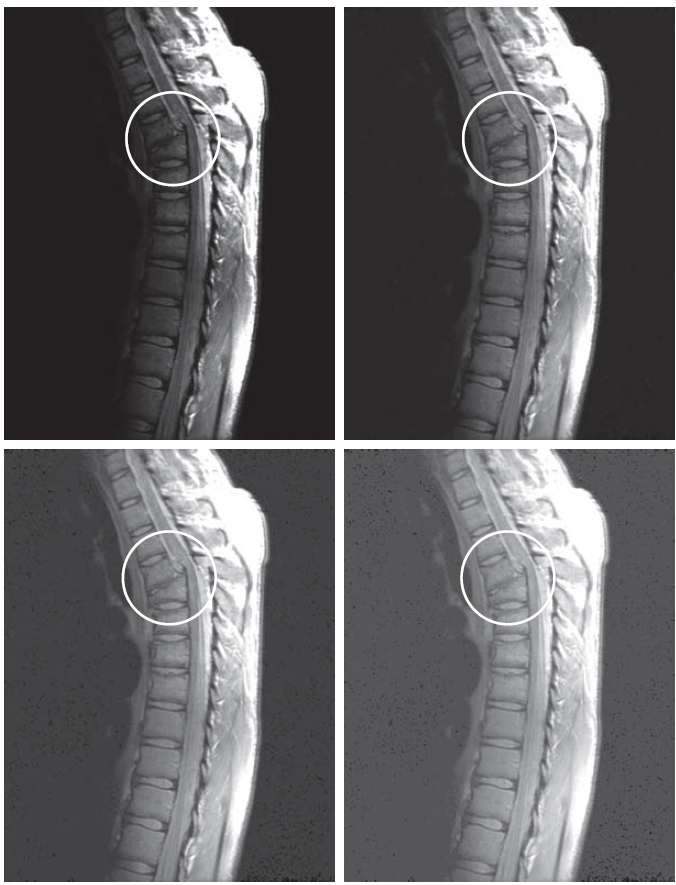
\includegraphics[width=0.4\linewidth]{figuras/Fig_3_8.png}
\caption{\tiny{(a) Magnetic
resonance
image (MRI) of a
fractured human
spine (the region
of the fracture is
enclosed by the
circle).
(b)–(d) Results of
applying the
transformation
in Eq. (3-5)
with c = 1 and
g = 0 6 . , 0.4, and
0.3, respectively.
(Original image
courtesy of Dr.
David R. Pickens,
Department of
Radiology and
Radiological
Sciences,
Vanderbilt
University
Medical Center.)}}
\end{figure}
\end{frame}

\begin{frame}{Aplicaci\'on A\'erea: Correcci\'on de Contraste (Fig. 3.9)}
\centering
\begin{figure}
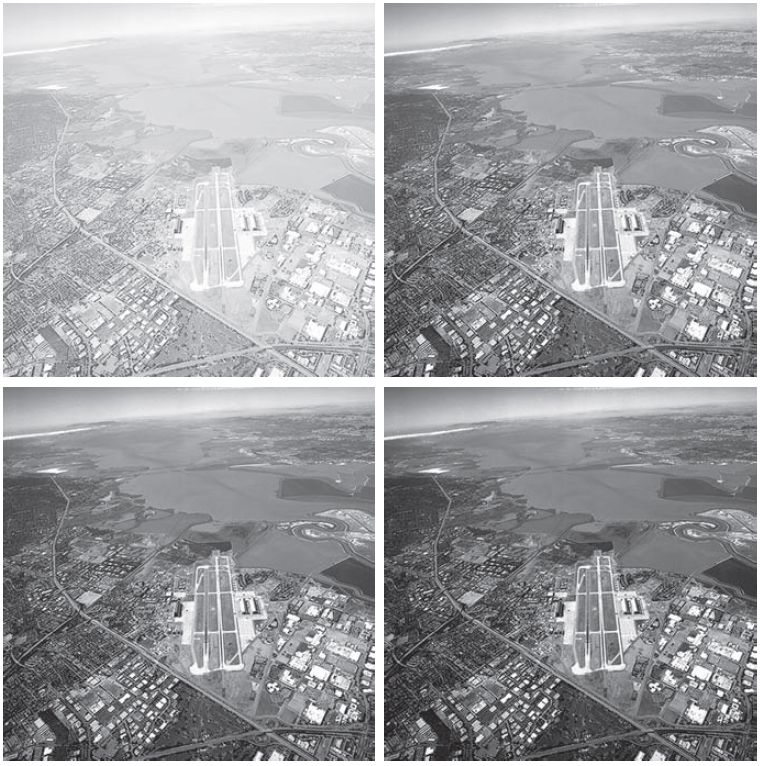
\includegraphics[width=0.5\linewidth]{figuras/Fig_3_9.png}
\caption{(a) Aerial image.
(b)–(d) Results
of applying the
transformation
in Eq. (3-5) with
g = 3 0 . , 4.0, and
5.0, respectively.
(c = 1 in all cases.)
(Original image
courtesy of
NASA.)}
\end{figure}
\end{frame}

% === RESUMEN ===
\begin{frame}{Resumen}
\begin{itemize}
    \item Transformaciones logar\'itmicas mejoran intensidades bajas.
    \item Transformaciones gamma permiten ajustes finos de brillo y contraste.
    \item Se aplican a espectros, dispositivos de visualizaci\'on e im\'agenes cl\'inicas.
\end{itemize}
\end{frame}

%%%%%%%%%%%%%%%%%%%%%%%%%%%%%%%%%%%%%%%%%%%%%%%%%%%%%%%%%%%%%%%%%%%%%%%%%%%%%%%%%%%%%%%%%%%%%%%%%%%%%%%%%%%%%%%%%%%%%%%%%%%%%%%%%%%%%%%%%%%%%%%%%%%%%%%%%%%

% --- Metadatos de la Presentación ---
\title{Descomposición en Planos de Bits (Bit-Plane Slicing)}
\subtitle{Análisis Visual de la Contribución de Bits}

% --- Configuraciones ---
%\setbeamertemplate{caption}[numbered]
%\captionsetup[subfigure]{labelformat=simple, textfont=it}
%\renewcommand{\thesubfigure}{(\alph{subfigure})}

% Colores TikZ
\definecolor{planeFill}{rgb}{0.6,0.75,0.9}
\definecolor{planeBorder}{rgb}{0.2,0.3,0.5}

% --- Diapositiva de Título ---
\begin{frame}
  \titlepage
\end{frame}

% --- Sección: Introducción ---
\section{Introducción al Bit-Plane Slicing}

\begin{frame}{Concepto Fundamental}
  \begin{block}{¿Qué es el Bit-Plane Slicing?}
    Es una técnica de procesamiento de imágenes que descompone una imagen digital en una serie de imágenes binarias, donde cada imagen corresponde a un plano de bits específico de los valores de intensidad de los píxeles.
  \end{block}

  \begin{itemize}
    \item Los valores de píxel en imágenes digitales (ej. escala de grises) son enteros representados por bits.
    \item Una imagen de 8 bits por píxel tiene valores de 0 a 255. Cada valor se representa con 8 bits.
    \item El Bit-Plane Slicing separa la contribución de cada posición de bit (0 a 7, o 1 a 8) a la apariencia general de la imagen.
  \end{itemize}
\end{frame}

\begin{frame}{Visualización de los Planos de Bits}
  \frametitle{Figura 3.13: Planos de Bits de una Imagen de 8 bits}
  \begin{figure}
    \centering
    \begin{tabular}{ccc}
      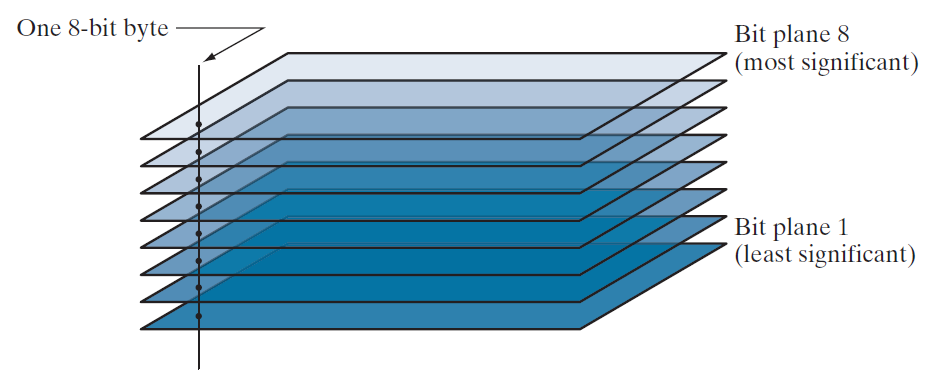
\includegraphics[width=0.7\textwidth]{figuras/Fig_3_13.png}
%      \includegraphics[width=0.3\textwidth]{placeholder_fig3_12b.png} &
%      \includegraphics[width=0.3\textwidth]{placeholder_fig3_12c.png} \\
    \end{tabular}
    \caption{Ilustración conceptual de cómo un byte de 8 bits que representa un píxel puede descomponerse en 8 planos de bits.}
  \end{figure}
  \begin{alertblock}{Significado}
    \begin{itemize}\footnotesize
      \item Plano 1 (LSB): Contiene el bit menos significativo de todos los píxeles.
      \item Plano 8 (MSB): Contiene el bit más significativo de todos los píxeles.
    \end{itemize}
  \end{alertblock}
\end{frame}

% --- Sección: Descomposición y Análisis ---
\section{Descomposición y Análisis}

\begin{frame}{Ejemplo: Imagen y sus Planos de Bits (Fig 3.14)}
  \frametitle{Figura 3.14: Imagen de 8 bits y sus Planos}

  \begin{figure}
    \centering
      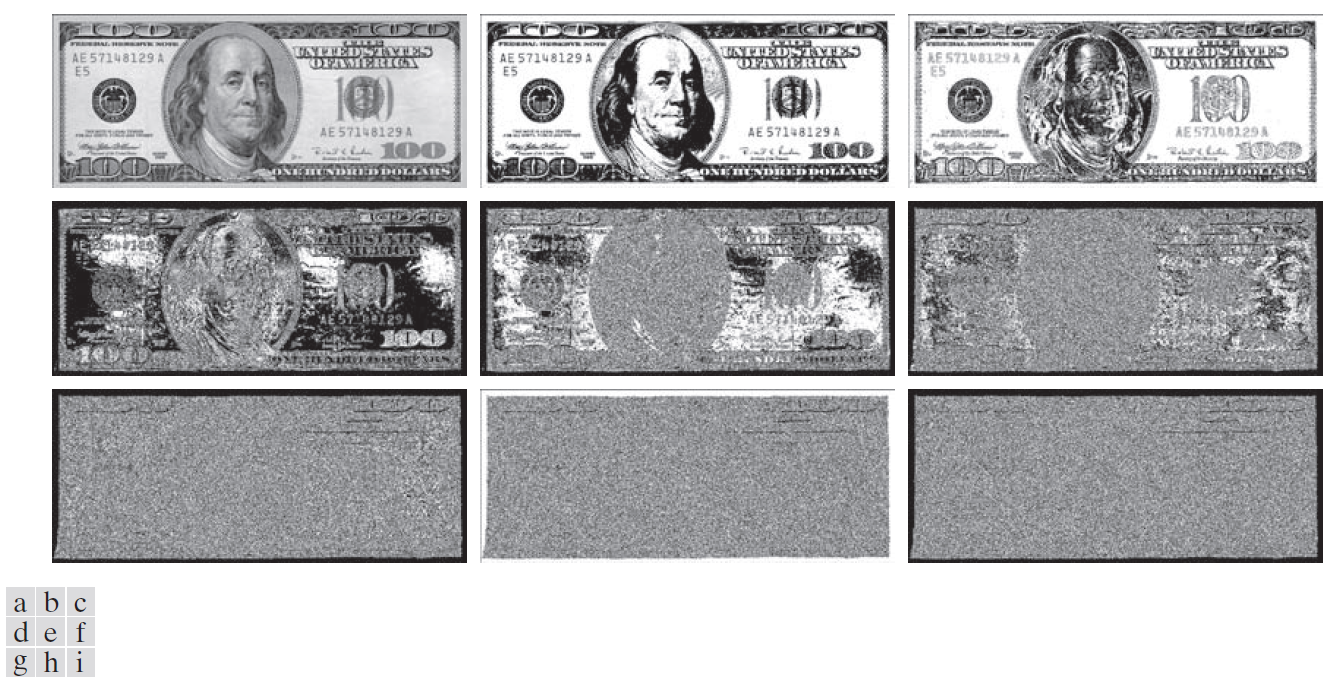
\includegraphics[width=\linewidth]{figuras/Fig_3_14.png}
    \caption{Una imagen de 8 bits (a) y sus ocho planos de bits (b-i), del más (Plano 8) al menos significativo (Plano 1).}
  \end{figure}
\end{frame}

\begin{frame}{Análisis Visual de los Planos}
  \begin{block}{Observaciones Clave (basado en Fig 3.14)}
    \begin{itemize}
      \item \textbf{Planos Superiores (MSB):} Los planos 8, 7, 6 y 5 contienen la mayor parte de la información visualmente significativa.
      \item \textbf{Planos Inferiores (LSB):} Los planos 4, 3, 2 y 1 aportan detalles sutiles de textura y a menudo parecen ruido.
      \item \textbf{Ejemplo (Valor 194):} 194 en binario es $11000010_2$, indicando bits MSB=1,1,0,0,0,0,1,0.
    \end{itemize}
  \end{block}
\end{frame}

% --- Sección: Reconstrucción y Aplicaciones ---
\section{Reconstrucción y Aplicaciones}

\begin{frame}{Reconstrucción a partir de Planos de Bits}
  \begin{block}{Principio de Reconstrucción}
    Una imagen $I(x,y)$ de $N$ bits se reconstruye sumando sus planos $B_n(x,y)$:
    \[
      I(x,y) = \sum_{n=1}^{N} B_n(x,y) \cdot 2^{n-1}
    \]
  \end{block}

  \begin{exampleblock}{Reconstrucción Aproximada}
    Usando solo planos de orden $k$ a $N$:
    \[
      I_{ap}(x,y) = \sum_{n=k}^{N} B_n(x,y) \cdot 2^{n-1}
    \]
  \end{exampleblock}
\end{frame}

\begin{frame}{Ejemplo: Reconstrucción con Menos Planos (Fig 3.15)}
  \frametitle{Figura 3.15: Reconstrucción usando Planos MSB}

  \begin{figure}[H]
    \centering
      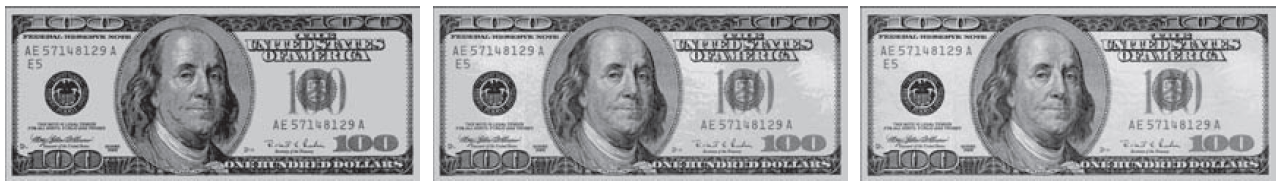
\includegraphics[width=\linewidth]{figuras/Fig_3_15.png}
    \caption{Reconstrucción usando diferentes combinaciones de planos MSB. a) Planos 8 y 7, b) Planos 8,7,6, c) Planos 8,7,6,5}
    \label{fig:reconstruction_example}
  \end{figure}
\end{frame}

\begin{frame}{Aplicaciones y Resumen}
  \begin{block}{Aplicaciones Principales}
    \begin{itemize}
      \item \textbf{Compresión:} Almacenar solo MSB (p.ej. 4 planos) reduce datos.
      \item \textbf{Análisis:} Cuantifica la importancia de cada bit.
      \item \textbf{Esteganografía:} Uso de LSB para ocultar información.
    \end{itemize}
  \end{block}

  \begin{exampleblock}{Resumen}
    \begin{itemize}
      \item Los planos MSB contienen la estructura esencial.
      \item Los LSB aportan detalles finos.
      \item Permite reconstrucciones aproximadas y aplicaciones en compresión y ocultación.
    \end{itemize}
  \end{exampleblock}
\end{frame}


%%%%%%%%%%%%%%%%%%%%%%%%%%%%%%%%%%%%%%%%%%%%%%%%%%%%%%%%%%%%%%%%%%%%%%%%%%%%%%%%%%%%%%%%%%%%%%%%%%%%%%%%%%%%%%%%%%%%%%%%%%%%%%%%%%%%%%%%%%%%%%%%%%%%%%%%%%%%%%%%%%%%

\title[[Procesamiento de Histogramas]{3.3 Procesamiento de Histogramas en Imágenes Digitales}
\subtitle{}
\author[Tu Nombre/Institución]{}
\date{}
\institute{}
% --- Diapositiva de título ---
\begin{frame}
  \titlepage
\end{frame}

\section{Definición y Propiedades del Histograma}

\begin{frame}{¿Qué es un Histograma?}
  \begin{block}{Definición}\footnotesize
    Sea $r_k$, $k=0,1,2,...,L-1$, las intensidades de una imagen digital de $L$ niveles, $f(x,y)$.
    \begin{itemize}
        \item El \textbf{histograma no normalizado} de $f$ se define como:
          \begin{equation}
            h(r_k) = n_k \quad \text{para } k=0,1,2,...,L-1
          \end{equation}
          donde $n_k$ es el número de píxeles en $f$ con intensidad $r_k$. Las subdivisiones de la escala de intensidad se llaman \textit{bins} del histograma.
        \item El \textbf{histograma normalizado} de $f$ se define como:
          \begin{equation}
            p(r_k) = \frac{h(r_k)}{MN} = \frac{n_k}{MN}
          \end{equation}
          donde $M$ y $N$ son el número de filas y columnas de la imagen.
    \end{itemize}
  \end{block}
  \begin{exampleblock}{Nota}\footnotesize
    Generalmente, se trabaja con histogramas normalizados. La suma de $p(r_k)$ para todos los valores de $k$ es siempre 1. Los componentes de $p(r_k)$ son estimaciones de las probabilidades de los niveles de intensidad.
  \end{exampleblock}
\end{frame}

\begin{frame}{Relación entre Histograma y Apariencia de la Imagen}
  \begin{columns}[T] % T para alinear por arriba
    \begin{column}{0.5\textwidth}
      \textbf{Imagen Oscura:}
      \begin{center}
      \begin{tikzpicture}[scale=0.6] % Escala ajustada
        \begin{axis}[
            ybar,
            xlabel={$r_k$ (intensidad)},
            ylabel={$p(r_k)$},
            xtick={0,0.5,1},
            xticklabels={0, L/2, L-1},
            ymin=0, ymax=0.4,
            bar width=6pt, % Ancho de barra ajustado
            width=\linewidth, height=4cm, % Altura ajustada
            title style={font=\footnotesize},
            xlabel style={font=\footnotesize},
            ylabel style={font=\footnotesize},
            ticklabel style={font=\scriptsize}
        ]
        \addplot coordinates {(0.1,0.3) (0.2,0.25) (0.3,0.15) (0.4,0.1) (0.5,0.05) (0.6,0.03) (0.7,0.02) (0.8,0.01)};
        \end{axis}
      \end{tikzpicture}
      \end{center}
      Bins concentrados en la parte inferior.
    \end{column}
    \begin{column}{0.5\textwidth}
      \textbf{Imagen Clara:}
      \begin{center}
      \begin{tikzpicture}[scale=0.6] % Escala ajustada
        \begin{axis}[
            ybar,
            xlabel={$r_k$ (intensidad)},
            ylabel={$p(r_k)$},
            xtick={0,0.5,1},
            xticklabels={0, L/2, L-1},
            ymin=0, ymax=0.4,
            bar width=6pt, % Ancho de barra ajustado
            width=\linewidth, height=4cm, % Altura ajustada
            title style={font=\footnotesize},
            xlabel style={font=\footnotesize},
            ylabel style={font=\footnotesize},
            ticklabel style={font=\scriptsize}
        ]
        \addplot coordinates {(0.2,0.01) (0.3,0.02) (0.4,0.03) (0.5,0.05) (0.6,0.1) (0.7,0.15) (0.8,0.25) (0.9,0.3)};
        \end{axis}
      \end{tikzpicture}
      \end{center}
      Bins concentrados en la parte superior.
    \end{column}
  \end{columns}
\end{frame}

\begin{frame}{Relación entre Histograma y Apariencia (Continuación)}
  \begin{columns}[T]
    \begin{column}{0.5\textwidth}
      \textbf{Bajo Contraste:}
      \begin{center}
      \begin{tikzpicture}[scale=0.6] % Escala ajustada
        \begin{axis}[
            ybar,
            xlabel={$r_k$ (intensidad)},
            ylabel={$p(r_k)$},
            xtick={0,0.5,1},
            xticklabels={0, L/2, L-1},
            ymin=0, ymax=0.5,
            bar width=6pt, % Ancho de barra ajustado
            width=\linewidth, height=4cm, % Altura ajustada
            title style={font=\footnotesize},
            xlabel style={font=\footnotesize},
            ylabel style={font=\footnotesize},
            ticklabel style={font=\scriptsize}
        ]
        \addplot coordinates {(0.4,0.1) (0.45,0.3) (0.5,0.4) (0.55,0.3) (0.6,0.1)};
        \end{axis}
      \end{tikzpicture}
      \end{center}
      Histograma estrecho, típicamente en el centro.
    \end{column}
    \begin{column}{0.5\textwidth}
      \textbf{Alto Contraste:}
      \begin{center}
      \begin{tikzpicture}[scale=0.6] % Escala ajustada
        \begin{axis}[
            ybar,
            xlabel={$r_k$ (intensidad)},
            ylabel={$p(r_k)$},
            xtick={0,0.5,1},
            xticklabels={0, L/2, L-1},
            ymin=0, ymax=0.2,
            bar width=6pt, % Ancho de barra ajustado
            width=\linewidth, height=4cm, % Altura ajustada
            title style={font=\footnotesize},
            xlabel style={font=\footnotesize},
            ylabel style={font=\footnotesize},
            ticklabel style={font=\scriptsize}
        ]
        \addplot coordinates {(0.1,0.1) (0.2,0.12) (0.3,0.08) (0.4,0.11) (0.5,0.09) (0.6,0.12) (0.7,0.1) (0.8,0.08) (0.9,0.11)};
        \end{axis}
      \end{tikzpicture}
      \end{center}
      Histograma amplio y distribuido.
    \end{column}
  \end{columns}
  \begin{block}{Observación}
    Una imagen con píxeles que ocupan todo el rango de intensidades y se distribuyen uniformemente tiende a tener alto contraste y mostrar gran detalle.
  \end{block}
\end{frame}

\begin{frame}
    \begin{figure}
    \centering
      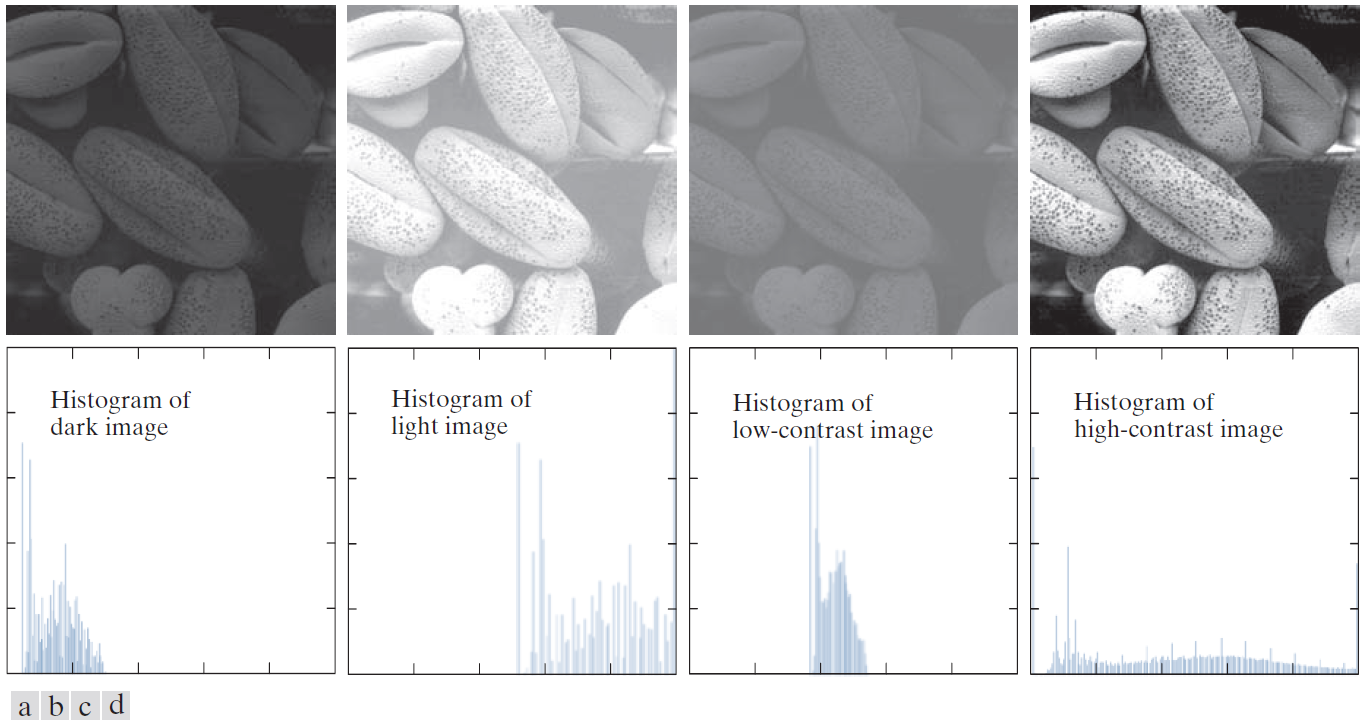
\includegraphics[width=0.8\linewidth]{figuras/Fig_3_16.png}
    \caption{Four image types and their corresponding histograms. (a) dark; (b) light; (c) low contrast; (d) high contrast. The horizontal axis of the histograms are values of $r_{k}$ and the vertical axis are values of $p(r_{k})$.}
    \end{figure}
\end{frame}

%------------------------------------------------------------
% Sección 2: Ecualización de Histograma
%------------------------------------------------------------
\title[Ecualización de Histograma]{Ecualización de Histograma}
\subtitle{}
\author[Tu Nombre/Institución]{}
\date{}
\institute{}
% --- Diapositiva de título ---
\begin{frame}
  \titlepage
\end{frame}


\begin{frame}{Transformaciones de Intensidad}
  \begin{block}{Mapeo de Intensidad}
    Consideramos transformaciones de la forma:
    \begin{equation}
      s = T(r), \quad 0 \le r \le L-1
    \end{equation}
    donde $r$ es la intensidad de entrada y $s$ es la intensidad de salida.
  \end{block}
  \pause
  \begin{alertblock}{Condiciones para $T(r)$}
    \begin{enumerate}[(a)]
      \item $T(r)$ es una función monotónicamente creciente en el intervalo $0 \le r \le L-1$.
      \item $0 \le T(r) \le L-1$ para $0 \le r \le L-1$.
    \end{enumerate}
    Para la transformación inversa $r = T^{-1}(s)$, la condición (a) se cambia a:
    \begin{enumerate}[(a')]
      \item $T(r)$ es una función \textbf{estrictamente} monotónicamente creciente.
    \end{enumerate}
  \end{alertblock}
\end{frame}

\begin{frame}{Funciones Monotónicas y Estrictamente Monotónicas}
    \begin{figure}
      \centering
      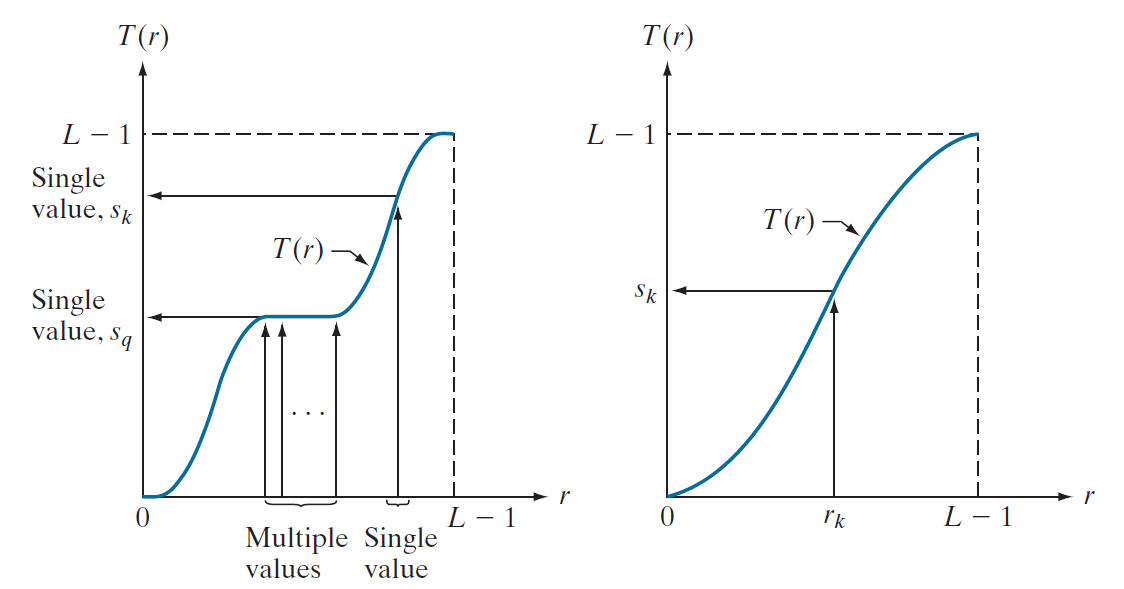
\includegraphics[width=0.8\linewidth]{figuras/Fig_3_17.png}
      \caption{a) Mapeo uno-a-uno o muchos-a-uno, b) Mapeo uno-a-uno. (a) Monotonic
increasing function,
showing how
multiple values can
map to a single
value. (b) Strictly
monotonic increasing
function. This is
a one-to-one mapping,
both ways.}
    \end{figure}
\end{frame}

\begin{frame}{PDF de la Intensidad Transformada (Caso Continuo)}\tiny
  \begin{block}{\footnotesize{Relación entre PDFs}}
    Si $p_r(r)$ es la Función de Densidad de Probabilidad (PDF) de las intensidades de entrada $r$, y $T(r)$ es conocida, continua y diferenciable, la PDF de las intensidades transformadas $s$ es:
    \begin{equation}
      p_s(s) = p_r(r) \left| \frac{dr}{ds} \right|
    \end{equation}
  \end{block}
  \pause
  \begin{alertblock}{\footnotesize{Transformación Clave para Ecualización}}
    Una transformación de particular importancia es:
    \begin{equation}
      s = T(r) = (L-1) \int_{0}^{r} p_r(w) dw
    \end{equation}
    donde $w$ es una variable dummy de integración. La integral es la Función de Distribución Acumulativa (CDF) de $r$.
  \end{alertblock}
  \pause
  \begin{exampleblock}{\footnotesize{Derivada $ds/dr$}}
    Usando la regla de Leibniz:
    \begin{equation}
      \frac{ds}{dr} = \frac{dT(r)}{dr} = (L-1) \frac{d}{dr} \left[ \int_{0}^{r} p_r(w) dw \right] = (L-1) p_r(r)
    \end{equation}
  \end{exampleblock}
\end{frame}

\begin{frame}{Resultado de la Ecualización (Caso Continuo)}\footnotesize
  Sustituyendo $\frac{dr}{ds} = \left(\frac{ds}{dr}\right)^{-1} = \frac{1}{(L-1)p_r(r)}$ en la Ec. (4):
  \begin{align}
    p_s(s) &= p_r(r) \left| \frac{1}{(L-1)p_r(r)} \right| \nonumber \\
           &= \frac{1}{L-1}, \quad \text{para } 0 \le s \le L-1
  \end{align}
  \begin{block}{\footnotesize{Resultado Fundamental}}
    La PDF resultante $p_s(s)$ es una \textbf{distribución uniforme}. Esto significa que la transformación de ecualización (Ec. 5) tiende a producir una imagen cuyas intensidades están distribuidas uniformemente en el rango $[0, L-1]$.
  \end{block}
  \begin{figure}
      \centering
      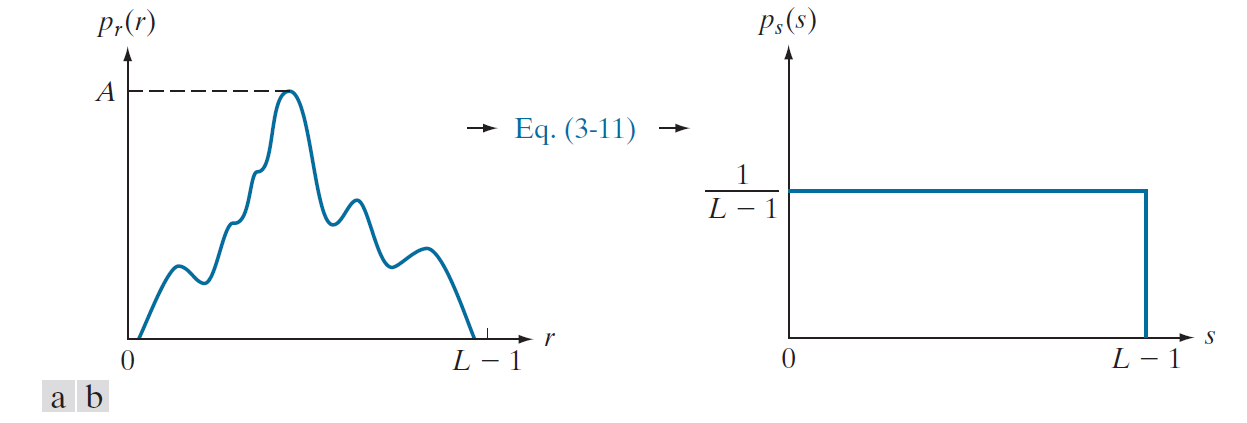
\includegraphics[width=0.55\linewidth]{figuras/Fig_3_18.png}
  \caption{\footnotesize{(a) An arbitrary PDF. (b) Result of applying Eq. (3-11) to the input PDF. The resulting PDF is always uniform, independently of the shape of the input.}}
  \end{figure}
\end{frame}

%------------------------------------------------------------
% Sección 3: Ecualización Discreta y Ejemplos
%------------------------------------------------------------
\section{Ecualización Discreta y Ejemplos}

\begin{frame}{Ecualización de Histograma para Imágenes Digitales (Discreta)}\footnotesize
  \begin{block}{\footnotesize{Probabilidad Discreta}}
    La probabilidad de ocurrencia del nivel de intensidad $r_k$ se aproxima por el histograma normalizado:
    \begin{equation}
      p_r(r_k) = \frac{n_k}{MN}
    \end{equation}
  \end{block}
  \pause
  \begin{alertblock}{\footnotesize{Transformación de Ecualización Discreta}}
    La forma discreta de la transformación (Ec. 5) es:
    \begin{equation}
      s_k = T(r_k) = (L-1) \sum_{j=0}^{k} p_r(r_j), \quad k=0,1,2,...,L-1
    \end{equation}
    Esta se conoce como ecualización de histograma o linealización de histograma. Los valores $s_k$ calculados se redondean al entero más cercano.
  \end{alertblock}
  \begin{exampleblock}{\footnotesize{Nota Importante}}
    Debido a la naturaleza discreta y el redondeo, el histograma resultante no es perfectamente plano en la práctica, pero tiende a estar más extendido.
  \end{exampleblock}
\end{frame}

\begin{frame}{Ejemplo 3.5: Mecánica de la Ecualización}\footnotesize
  Supongamos una imagen de 3 bits ($L=8$, intensidades $0..7$) de $64 \times 64$ píxeles ($MN=4096$).\\
  \textbf{Tabla 3.1: Distribución de intensidad e histograma}\tiny\\
  \centering
  \resizebox{0.9\textwidth}{!}{%
  \begin{tabular}{|c|c|c||c|c|c|}
    \hline
    $r_k$ & $n_k$ & $p_r(r_k) = n_k/MN$ & $r_k$ & $n_k$ & $p_r(r_k) = n_k/MN$ \\
    \hline
    $r_0=0$ & 790 & 0.19 & $r_4=4$ & 329 & 0.08 \\
    $r_1=1$ & 1023 & 0.25 & $r_5=5$ & 245 & 0.06 \\
    $r_2=2$ & 850 & 0.21 & $r_6=6$ & 122 & 0.03 \\
    $r_3=3$ & 656 & 0.16 & $r_7=7$ & 81 & 0.02 \\
    \hline
  \end{tabular}
  }
  \vspace{0.5em} % Espacio reducido
  \pause\\
  \footnotesize{Aplicando Ec. (8) ($L-1=7$):}
  \begin{footnotesize} % Reducir tamaño de fuente para la lista
  \begin{itemize}
    \item $s_0 = 7 \sum_{j=0}^{0} p_r(r_j) = 7 p_r(r_0) = 7 \times 0.19 = 1.33 \rightarrow \mathbf{1}$
    \item $s_1 = 7 \sum_{j=0}^{1} p_r(r_j) = 7 (p_r(r_0) + p_r(r_1)) = 7 \times (0.19+0.25) = 3.08 \rightarrow \mathbf{3}$
    \item $s_2 = 7 \sum_{j=0}^{2} p_r(r_j) = 7 (0.19+0.25+0.21) = 7 \times 0.65 = 4.55 \rightarrow \mathbf{5}$
    \item $s_3 = 7 (0.65+0.16) = 7 \times 0.81 = 5.67 \rightarrow \mathbf{6}$
    \item $s_4 = 7 (0.81+0.08) = 7 \times 0.89 = 6.23 \rightarrow \mathbf{6}$
    \item $s_5 = 7 (0.89+0.06) = 7 \times 0.95 = 6.65 \rightarrow \mathbf{7}$
    \item $s_6 = 7 (0.95+0.03) = 7 \times 0.98 = 6.86 \rightarrow \mathbf{7}$
    \item $s_7 = 7 (0.98+0.02) = 7 \times 1.00 = 7.00 \rightarrow \mathbf{7}$
  \end{itemize}
  \end{footnotesize}
\end{frame}

\begin{frame}{Ejemplo 3.5: Histogramas y Función de Transformación}\footnotesize
  \begin{columns}[T]
    \begin{column}{0.33\textwidth}
      \textbf{(a) Histograma Original}
      \begin{tikzpicture}[scale=1.0, transform shape] % Escala ajustada
        \begin{axis}[
            ybar,
            xlabel={$r_k$}, ylabel={$p_r(r_k)$},
            symbolic x coords={0,1,2,3,4,5,6,7},
            xtick=data,
            ymin=0, ymax=0.3,
            bar width=4pt, % Ancho de barra ajustado
            width=\linewidth, height=3.2cm, % Altura ajustada
            title style={font=\tiny},xlabel style={font=\tiny},ylabel style={font=\tiny},ticklabel style={font=\tiny}
        ]
        \addplot coordinates {(0,0.19) (1,0.25) (2,0.21) (3,0.16) (4,0.08) (5,0.06) (6,0.03) (7,0.02)};
        \end{axis}
      \end{tikzpicture}
    \end{column}
    \begin{column}{0.33\textwidth}
      \textbf{(b) Función $T(r_k)$}
      \begin{tikzpicture}[scale=1.0, transform shape] % Escala ajustada
        \begin{axis}[
            xlabel={$r_k$}, ylabel={$s_k = T(r_k)$},
            xtick={0,1,...,7}, ytick={0,1,...,7},
            ymin=0, ymax=7,
            width=\linewidth, height=3.2cm, % Altura ajustada
            const plot,
            title style={font=\tiny},xlabel style={font=\tiny},ylabel style={font=\tiny},ticklabel style={font=\tiny}
        ]
        \addplot+[const plot, mark=*] coordinates {(0,1.33) (1,3.08) (2,4.55) (3,5.67) (4,6.23) (5,6.65) (6,6.86) (7,7.00) (8,7.00)};
        \end{axis}
      \end{tikzpicture}
    \end{column}
    \begin{column}{0.33\textwidth}
      \textbf{(c) Histograma Ecualizado}
      % (Valores $s_k$ redondeados: 1, 3, 5, 6, 6, 7, 7, 7) % Texto movido o acortado si es necesario
      \begin{tikzpicture}[scale=1.0, transform shape] % Escala ajustada
        \begin{axis}[
            ybar,
            xlabel={$s_k$}, ylabel={$p_s(s_k)$},
            symbolic x coords={0,1,2,3,4,5,6,7},
            xtick=data,
            ymin=0, ymax=0.3,
            bar width=4pt, % Ancho de barra ajustado
            width=\linewidth, height=3.2cm, % Altura ajustada
            title style={font=\tiny},xlabel style={font=\tiny},ylabel style={font=\tiny},ticklabel style={font=\tiny}
        ]
        \addplot coordinates {(1,0.19) (3,0.25) (5,0.21) (6,0.2404) (7,0.1093)};
        \end{axis}
      \end{tikzpicture}
    \end{column}
  \end{columns}
  \begin{block}{\footnotesize{Observación del Ejemplo}}
  \footnotesize % Fuente más pequeña para el bloque
  El histograma ecualizado (c) muestra cómo las intensidades se han redistribuido, ocupando un rango más amplio y tendiendo a una distribución más uniforme, aunque no perfectamente plana. Algunos niveles de intensidad originales se mapean al mismo nivel de salida.
  \end{block}
\end{frame}

\begin{frame}{Ventajas de la Ecualización de Histograma}
  \begin{itemize}
    \item \textbf{Mejora del Contraste:} Generalmente, la ecualización extiende el histograma de la imagen de entrada, resultando en un realce del contraste.
    \item \textbf{Automática:} El proceso se basa enteramente en la información extraída de la imagen dada (su histograma), sin necesidad de parámetros externos.
    \item \textbf{Adaptativa:} Se adapta a las características de cada imagen.
  \end{itemize}
  \pause
  \begin{alertblock}{Transformación Inversa}
    La transformación inversa de $s$ a $r$ se denota como:
    \begin{equation}
      r_k = T^{-1}(s_k)
    \end{equation}
    Esta transformación es importante para técnicas como el \textit{histogram matching} (especificación de histograma). Para que sea única, todas las intensidades deben estar presentes en la imagen original (histograma sin bins vacíos).
  \end{alertblock}
\end{frame}


%------------------------------------------------------------
% Sección 4: Resumen y Aplicaciones
%------------------------------------------------------------
\section{Resumen y Aplicaciones}

\begin{frame}{Resumen Clave}
  \begin{itemize}
    \item El \textbf{histograma} de una imagen describe la distribución de sus niveles de intensidad.
    \item La forma del histograma está directamente relacionada con la \textbf{apariencia visual} de la imagen (oscura, clara, contraste).
    \item La \textbf{ecualización de histograma} es una técnica que busca transformar una imagen para que su histograma sea lo más uniforme posible.
    \item \textbf{Teoría (Continua):} Se basa en la CDF de la PDF de intensidades, resultando en una PDF de salida teóricamente uniforme.
    \item \textbf{Práctica (Discreta):} Se usa la CDF del histograma normalizado. El resultado no es perfectamente plano pero tiende a mejorar el contraste significativamente.
    \item Es un método \textbf{automático y adaptativo} para el realce de contraste.
  \end{itemize}
\end{frame}

\begin{frame}{Aplicaciones del Procesamiento de Histogramas}
  \begin{block}{Usos Comunes}
    El procesamiento de histogramas, y en particular la ecualización, es fundamental en:
  \end{block}
    \begin{itemize}
        \item Realce de contraste en imágenes médicas (rayos X, resonancias magnéticas).
        \item Mejora de fotografías subexpuestas o sobreexpuestas.
        \item Preprocesamiento en sistemas de visión por computadora para mejorar la detectabilidad de características.
        \item Normalización de imágenes para comparación o análisis.
        \item Segmentación de imágenes (umbralización basada en histograma).
    \end{itemize}
\end{frame}

%------------------------------------------------------------
% Diapositiva Final
%------------------------------------------------------------
\begin{frame}
\begin{figure}
    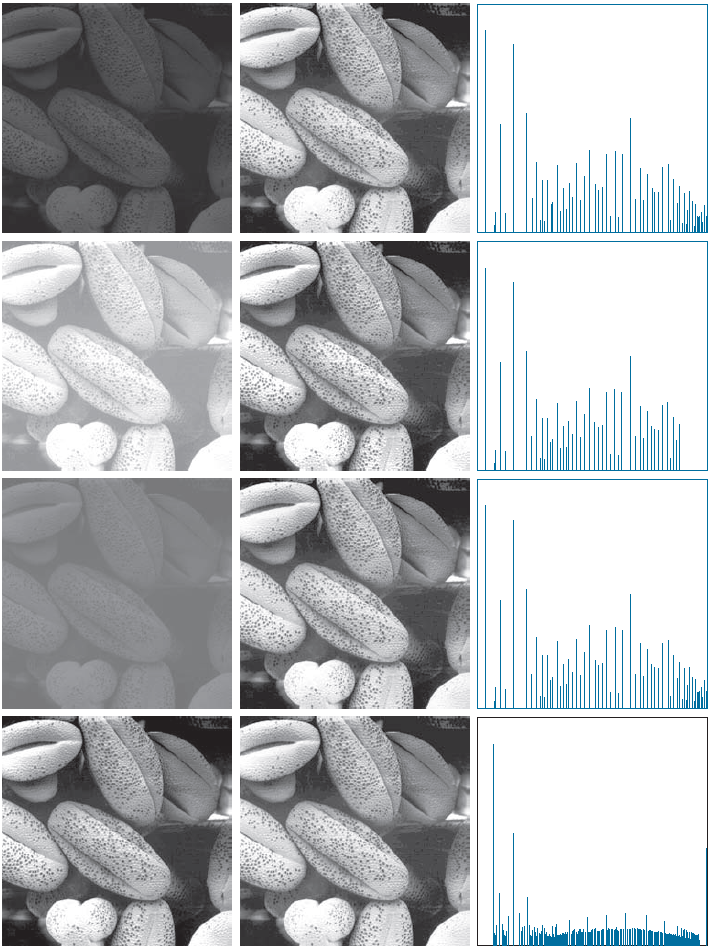
\includegraphics[width=0.45\linewidth]{figuras/Fig_3_20.png}
    \caption{\footnotesize{Left column: Images from Fig. 3.16. Center column: Corresponding histogram-equalized images. Right column: histograms of the images in the center column (compare with the histograms in Fig. 3.16).}}
\end{figure}
\end{frame}


%%%%%%%%%%%%%%%%%%%%%%%%%%%%%%%%%%%%%%%%%%%%%%%%%%%%%%%%%%%%%%%%%%%%%%%%%%%%%%%%%%%%%%%%%%%%%%%%%%%%%%%%%%%%%%%%%%%%%%%%%%%%%%%%%%%%%%%%%%%%%%%%%%%%%%%%%%%%%%%%%%%%%%%%%%%%%%%%%%%%%%%%%%%

\title[Especificación de Histograma (Matching)]{Especificación de Histograma (Matching)}
\subtitle{}
\author[Tu Nombre/Institución]{}
\date{}
\institute{}
% --- Diapositiva de título ---
\begin{frame}
  \titlepage
\end{frame}

\begin{frame}{Introducción a la Especificación de Histograma}
 \begin{block}{Concepto}
  La ecualización de histograma busca un histograma de salida uniforme. A veces, se desea especificar una forma particular para el histograma de la imagen procesada. Este método se llama \textbf{especificación de histograma} o \textbf{histogram matching}.
 \end{block}
 \pause
 \begin{exampleblock}{Variables}
  \begin{itemize}
   \item $r$: intensidades de la imagen de entrada (PDF $p_r(r)$).
   \item $z$: intensidades de la imagen de salida (PDF deseada $p_z(z)$).
  \end{itemize}
 \end{exampleblock}
\end{frame}

\begin{frame}{Especificación de Histograma: Caso Continuo}
 \begin{alertblock}{Transformaciones Fundamentales}
  Sea $s$ una variable aleatoria tal que (repetición de Ec. \eqref{eq:Tr_continuo}):
  \begin{equation}
   s = T(r) = (L-1) \int_{0}^{r} p_r(w) dw \label{eq:spec_Tr}
  \end{equation}
  Definimos una función $G(z)$ sobre la variable $z$:
  \begin{equation}
   G(z) = (L-1) \int_{0}^{z} p_z(v) dv = s \label{eq:spec_Gz}
  \end{equation}
  De las ecuaciones anteriores, $G(z) = s = T(r)$, por lo tanto:
  \begin{equation}
   z = G^{-1}(s) = G^{-1}[T(r)] \label{eq:spec_z_transform}
  \end{equation}
 \end{alertblock}
\end{frame}

\begin{frame}{Procedimiento de Especificación (Continuo)}
 \begin{enumerate}
  \item Obtener $p_r(r)$ de la imagen de entrada y usarla en Ec. \eqref{eq:spec_Tr} para hallar $T(r)$.
  \item Usar la PDF especificada $p_z(z)$ en Ec. \eqref{eq:spec_Gz} para obtener la función $G(z)$.
  \item Calcular la transformación inversa $z = G^{-1}(s)$. Este es el mapeo de $s$ a $z$.
  \item Obtener la imagen de salida:
        \begin{itemize}
            \item Ecualizar la imagen de entrada usando Ec. \eqref{eq:spec_Tr} (valores $s$).
            \item Para cada píxel con valor $s$, aplicar el mapeo inverso $z=G^{-1}(s)$ para obtener el píxel correspondiente en la imagen de salida.
        \end{itemize}
 \end{enumerate}
 \begin{exampleblock}{Nota}
  Encontrar expresiones analíticas para $G^{-1}$ puede ser no trivial.
 \end{exampleblock}
\end{frame}

\begin{frame}{Funciones de Transformación (Ilustración Conceptual de Fig. 3.21)}\footnotesize
    \begin{block}{Mapeo $s=T(r)$ para Ecualización}
    La Figura 3.21 del texto fuente muestra ejemplos de funciones de transformación $s=T(r)$ obtenidas para diferentes imágenes. Estas funciones mapean los niveles de intensidad originales $r$ a los niveles de intensidad $s$ de una imagen ecualizada.
    \end{block}
    \centering
    Ilustración conceptual de funciones de transformación $s=T(r)$.
    \begin{tikzpicture}[scale=0.7]
        \begin{axis}[
            xlabel={Valores de intensidad originales $r$},
            ylabel={Valores de intensidad ecualizados $s$},
            xmin=0, xmax=255, ymin=0, ymax=255,
            width=0.8\textwidth, height=6cm,
            legend pos=north west,
            title style={font=\footnotesize}, xlabel style={font=\footnotesize}, ylabel style={font=\footnotesize}, ticklabel style={font=\scriptsize}
        ]
        % Curva ejemplo para imagen oscura -> más clara
        \addplot[smooth, thick, blue, domain=0:255] {255 * (x/255)^(0.5)} node[pos=0.8, pin=45:{\tiny $T_1(r)$ (ej. oscura)}]{};
        % Curva ejemplo para imagen ya con buen contraste (casi lineal)
        \addplot[smooth, thick, red, domain=0:255] {x} node[pos=0.8, pin=-45:{\tiny $T_2(r)$ (ej. alto contraste)}]{};
        % Curva ejemplo para imagen clara -> más oscura (menos común en ecualización simple)
        \addplot[smooth, thick, green!50!black, domain=0:255] {255 * (x/255)^(2)} node[pos=0.3, pin=135:{\tiny $T_3(r)$ (ej. clara)}]{};

        \draw[dashed] (axis cs:64,0) -- (axis cs:64, {255 * (64/255)^(0.5)}) node[left, font=\tiny]{$s_k$};
        \node[below, font=\tiny] at (axis cs:64,0) {$r_k$};
        \end{axis}
    \end{tikzpicture}
\end{frame}

\begin{frame}{Especificación de Histograma: Caso Discreto}\footnotesize
 \begin{block}{Formulación Discreta}
  La Ec. \eqref{eq:spec_Tr} en forma discreta es la transformación de ecualización (Ec. \eqref{eq:Tr_discreta}):
  \begin{equation}
   s_k = T(r_k) = (L-1) \sum_{j=0}^{k} p_r(r_j) \label{eq:spec_sk_discreta}
  \end{equation}
  \pause
  Dado $s_k$, la formulación discreta de Ec. \eqref{eq:spec_Gz} implica calcular:
  \begin{equation}
   G(z_q) = (L-1) \sum_{i=0}^{q} p_z(z_i) \label{eq:spec_Gzq_discreta}
  \end{equation}
  para un valor $q$ tal que $G(z_q) \approx s_k$. \pause Los valores $z_q$ deseados se obtienen de la transformación inversa:
  \begin{equation}
   z_q = G^{-1}(s_k) \label{eq:spec_zq_inversa}
  \end{equation}
 \end{block}
 \begin{exampleblock}{Nota}
  En la práctica, no se calcula $G^{-1}$ directamente. Se usan tablas de consulta (look-up tables).
 \end{exampleblock}
\end{frame}

\begin{frame}{Procedimiento de Especificación (Discreto)}
 \footnotesize % Reducir tamaño de fuente para esta diapositiva
 \begin{enumerate}
  \item Calcular el histograma $p_r(r_k)$ de la imagen de entrada. Usarlo en Ec. \eqref{eq:spec_sk_discreta} para mapear las intensidades de entrada $r_k$ a las intensidades $s_k$ de la imagen ecualizada. Redondear $s_k$ al rango $[0, L-1]$.
  \item Calcular todos los valores de la función $G(z_q)$ usando Ec. \eqref{eq:spec_Gzq_discreta} para $q=0,1,...,L-1$, donde $p_z(z_i)$ son los valores del histograma especificado. Redondear los valores de $G(z_q)$ al rango $[0, L-1]$. Almacenar estos $G(z_q)$ en una tabla de consulta.
  \item Para cada valor de $s_k$ ($k=0,1,...,L-1$), usar los valores almacenados de $G(z_q)$ del Paso 2 para encontrar el valor $z_q$ tal que $G(z_q)$ sea el más cercano a $s_k$. Almacenar estos mapeos de $s_k \rightarrow z_q$. Si hay múltiples $z_q$ que dan la misma cercanía, se elige el menor por convención.
  \item Formar la imagen con histograma especificado mapeando cada píxel ecualizado con valor $s_k$ al correspondiente píxel con valor $z_q$ en la imagen de salida, usando los mapeos del Paso 3.
 \end{enumerate}
 \begin{block}{Observación}
  El paso intermedio de ecualizar la imagen es conceptual y puede omitirse combinando $T$ y $G^{-1}$.
 \end{block}
\end{frame}


%------------------------------------------------------------
% Sección 5: Resumen y Aplicaciones (General)
%------------------------------------------------------------
\section{Resumen y Aplicaciones (General)}

\begin{frame}{Resumen Clave}
  \begin{itemize}
    \item El \textbf{histograma} describe la distribución de intensidades.
    \item La \textbf{ecualización} busca un histograma uniforme, mejorando el contraste automáticamente.
    \item La \textbf{especificación (matching)} permite dar una forma deseada al histograma de salida.
    \item Ambas técnicas se basan en la CDF (o suma acumulada del histograma).
    \item Las implementaciones discretas involucran redondeo y aproximaciones.
  \end{itemize}
\end{frame}

\begin{frame}{Aplicaciones del Procesamiento de Histogramas}
  \begin{block}{Usos Comunes}
    El procesamiento de histogramas es fundamental en:
  \end{block}
    \begin{itemize}
        \item Realce de contraste (ecualización).
        \item Lograr una apariencia específica (especificación).
        \item Normalización de imágenes para comparación.
        \item Segmentación (umbralización).
        \item Aplicaciones médicas, fotografía, visión por computadora.
    \end{itemize}
\end{frame}

%%%%%%%%%%%%%%%%%%%%%%%%%%%%%%%%%%%%%%%%%%%%%%%%%%%%%%%%%%%%%%%%%%%%%%%%%%%%%%%%%%%%%%%%%%%%%%%%%%%%%%%%%%%%%%%%%%%%%%%%%%%%%%%%%%%%%%%%%%%%%%%%%%%%%%%%%%%%%%%%%%%%%%%%%%%%%%%%%%%%%%%%%%%%%%%%%%%%%%%

\title[Especificación de Histograma (Matching)]{Ejemplo 3.7 Especificación de Histograma (Matching)}
\subtitle{}
\author[Tu Nombre/Institución]{}
\date{}
\institute{}
% --- Diapositiva de título ---
\begin{frame}
  \titlepage
\end{frame}


\begin{frame}{Especificación de Histogramas}
  \begin{block}{Definición}
    La especificación de histogramas (o igualación de histogramas) es una técnica de procesamiento de imágenes que busca transformar el histograma de una imagen para que coincida (aproximadamente) con un histograma especificado o deseado.
  \end{block}

  \begin{itemize}
    \item Permite controlar de forma más precisa la distribución de las intensidades de los píxeles.
    \item Útil para mejorar el contraste de forma selectiva o para comparar imágenes procesadas bajo diferentes condiciones de iluminación.
  \end{itemize}

  \begin{alertblock}{Objetivo del Ejemplo}
    Ilustrar la mecánica de la especificación de histogramas, transformando una imagen (cuyo histograma ecualizado es conocido) para que su nuevo histograma se aproxime a uno especificado.
  \end{alertblock}
\end{frame}

% ========== Sección: Datos Iniciales y Pasos del Proceso ==========
\section{Datos Iniciales y Pasos del Proceso}

\begin{frame}{Paso 1: Histograma Ecualizado de la Imagen Original ($s_k$)}
  Se asume que se parte de una imagen cuyo histograma ya ha sido ecualizado (o se conocen los valores $s_k$ resultantes de la ecualización). Estos valores $s_k = T(r_k)$ representan los niveles de gris transformados de la imagen original.

  \begin{exampleblock}{Valores $s_k$ (del Ejemplo 3.5 del libro de texto)}
    \footnotesize % Reducir tamaño de fuente para esta lista
    Para una imagen de 8 bits (niveles $0-7$), los valores $s_k$ obtenidos tras la ecualización son:
    \begin{multicols}{2} % Usar dos columnas para la lista
        \begin{itemize}
            \item $s_0 = 1$
            \item $s_1 = 3$
            \item $s_2 = 5$
            \item $s_3 = 6$
            \item $s_4 = 6$
            \item $s_5 = 7$
            \item $s_6 = 7$
            \item $s_7 = 7$
        \end{itemize}
    \end{multicols}
    Estos son los valores que se buscará mapear a nuevos niveles $z_q$.
  \end{exampleblock}
\end{frame}

\begin{frame}{Paso 2: Histograma Especificado ($P_z(z_q)$)}
  Se define el histograma deseado $P_z(z_q)$ para los niveles de intensidad $z_q$.

  \begin{block}{Tabla 3.2 (Parcial): Histograma Especificado}
  \centering\footnotesize % Reducir tamaño de fuente para la tabla
  \begin{tabular}{cc}
    \toprule
    $z_q$ & Specified $P_z(z_q)$ \\
    \midrule
    $z_0 = 0$ & 0.00 \\
    $z_1 = 1$ & 0.00 \\
    $z_2 = 2$ & 0.00 \\
    $z_3 = 3$ & 0.15 \\
    $z_4 = 4$ & 0.20 \\
    $z_5 = 5$ & 0.30 \\
    $z_6 = 6$ & 0.20 \\
    $z_7 = 7$ & 0.15 \\
    \bottomrule
  \end{tabular}
  \end{block}
  Estos valores son los que se usarán para calcular la función de transformación $G(z_q)$.
\end{frame}

\begin{frame}{Paso 3: Calcular la Función de Transformación $G(z_q)$}
\frametitle{Paso 3: Calcular $G(z_q)$} % Título más corto
  La función $G(z_q)$ se calcula a partir de $P_z(z_q)$:
  \begin{equation}
    G(z_q) = (L-1) \sum_{j=0}^{q} P_z(z_j) \label{eq:Gzq_calc}
  \end{equation}
  donde $L=8$, por lo tanto $L-1=7$.

  \begin{columns}[T,onlytextwidth] % onlytextwidth ayuda a controlar el ancho
    \begin{column}{0.5\textwidth}
      \footnotesize % Reducir tamaño
      \textbf{Valores $G(z_q)$ (fraccionales):}
      \begin{itemize}
        \item $G(z_0) = 0.00$
        \item $G(z_1) = 0.00$
        \item $G(z_2) = 0.00$
        \item $G(z_3) = 1.05$
        \item $G(z_4) = 2.45$
        \item $G(z_5) = 4.55$
        \item $G(z_6) = 5.95$
        \item $G(z_7) = 7.00$
      \end{itemize}
    \end{column}
    \begin{column}{0.5\textwidth}
      \footnotesize % Reducir tamaño
      \textbf{$G(z_q)$ redondeados (Tabla 3.3):}
        \centering % Centrar tabla
        \begin{tabular}{cc}
            \toprule
            $z_q$ & $G(z_q)$ \\
            \midrule
            0 & 0 \\
            1 & 0 \\
            2 & 0 \\
            3 & 1 \\
            4 & 2 \\
            5 & 5 \\
            6 & 6 \\
            7 & 7 \\
            \bottomrule
        \end{tabular}
    \end{column}
  \end{columns}
\end{frame}

\begin{frame}{Paso 4: Mapeo de $s_k$ a $z_q$}\footnotesize
\frametitle{Paso 4: Mapeo $s_k \rightarrow z_q$} % Título más corto
  Para cada $s_k$, se busca $z_q$ tal que $G(z_q)$ sea el más cercano a $s_k$.

  \begin{block}{\footnotesize{Regla de Mapeo}}
    $s_k \rightarrow z_q \quad \text{tal que } |s_k - G(z_q)| \text{ es mínimo.}$
  \end{block}

  \begin{exampleblock}{\footnotesize{Tabla 3.4: Mapeo de $s_k$ a $z_q$}}
    \tiny % Reducir tamaño
    Valores $s_k$ únicos: $\{1, 3, 5, 6, 7\}$.
    \begin{itemize}
        \item $s_k = 1 \rightarrow z_3=3$ (ya que $G(z_3)=1$)
        \item $s_k = 3 \rightarrow z_4=4$ (ya que $G(z_4)=2$ es el más cercano)
        \item $s_k = 5 \rightarrow z_5=5$ (ya que $G(z_5)=5$)
        \item $s_k = 6 \rightarrow z_6=6$ (ya que $G(z_6)=6$)
        \item $s_k = 7 \rightarrow z_7=7$ (ya que $G(z_7)=7$)
    \end{itemize}
    \centering
    \begin{tabular}{ccc}
        \toprule
        $s_k$ & $\rightarrow$ & $z_q$ \\
        \midrule
        1 & $\rightarrow$ & 3 \\
        3 & $\rightarrow$ & 4 \\
        5 & $\rightarrow$ & 5 \\
        6 & $\rightarrow$ & 6 \\
        7 & $\rightarrow$ & 7 \\
        \bottomrule
    \end{tabular}
  \end{exampleblock}
\end{frame}

% ========== Sección: Resultados Gráficos ==========
\section{Resultados Gráficos (Figura 3.22 del libro)}

\begin{frame}{Figura 3.22 (b): Histograma Especificado $P_z(z_q)$}
  \begin{figure}
  \centering
  \begin{tikzpicture} % No es necesario scale si se ajusta width/height en axis
    \begin{axis}[
        ybar interval,
        xlabel={$z_q$ (Nivel de intensidad)},
        ylabel={$P_z(z_q)$}, % Más corto
        ymin=0, ymax=0.35,
        xmin=-0.5, xmax=8.5,
        xtick={0,1,2,3,4,5,6,7},
        ytick={0,0.05,0.10,0.15,0.20,0.25,0.30},
        width=0.5\textwidth, % Reducir ancho
        height=5cm,         % Reducir altura
        title={Fig. 3.22(b) Histograma Especificado},
        bar width=6pt,      % Barras un poco más delgadas
      ]
      \addplot coordinates {
        (0, 0.00) (1, 0.00) (2, 0.00) (3, 0.15) (4, 0.20) (5, 0.30) (6, 0.20) (7, 0.15) (8, 0)
      };
    \end{axis}
  \end{tikzpicture}
  \caption{\footnotesize Histograma que se desea obtener.}
  \end{figure}
\end{frame}

\begin{frame}{Figura 3.22 (c): Función de Transformación $G(z_q)$}
  \begin{figure}
  \centering
  \begin{tikzpicture}
    \begin{axis}[
        xlabel={$z_q$ (Nivel de intensidad)},
        ylabel={$G(z_q)$}, % Más corto
        ymin=-0.5, ymax=7.5,
        xmin=-0.5, xmax=7.5,
        xtick={0,1,2,3,4,5,6,7},
        ytick={0,1,2,3,4,5,6,7},
        width=0.8\textwidth, % Reducir ancho
        height=5cm,         % Reducir altura
        title={Fig. 3.22(c) Función de Transformación (Redondeada)},
        grid=major,
      ]
      \addplot[const plot, mark=*, blue, thick] coordinates {
        (0,0) (1,0) (2,0) (3,1) (4,2) (5,5) (6,6) (7,7) (7.1, 7)
      };
      \addplot[only marks, mark=*, blue] coordinates {
        (0,0) (1,0) (2,0) (3,1) (4,2) (5,5) (6,6) (7,7)
      };
    \end{axis}
  \end{tikzpicture}
  \caption{\footnotesize Función de transformación $G(z_q)$ obtenida y redondeada.}
  \end{figure}
\end{frame}


\begin{frame}{Figura 3.22 (d): Histograma Resultante}
  \begin{block}{\footnotesize Tabla 3.2 (Parcial): Histograma Actual Obtenido} % Fuente más pequeña para el título del bloque
  \centering\scriptsize % Fuente aún más pequeña para esta tabla
  \begin{tabular}{cc}
    \toprule
    $z_q$ & Actual $P_z(z_q)$ \\
    \midrule
    $z_0 = 0$ & 0.00 \\ $z_1 = 1$ & 0.00 \\
    $z_2 = 2$ & 0.00 \\ $z_3 = 3$ & 0.19 \\
    $z_4 = 4$ & 0.25 \\ $z_5 = 5$ & 0.21 \\
    $z_6 = 6$ & 0.24 \\ $z_7 = 7$ & 0.11 \\
    \bottomrule
  \end{tabular}
  \end{block}

  \begin{figure}\footnotesize
  \centering
  \begin{tikzpicture}
    \begin{axis}[
        ybar interval,
        xlabel={$z_q$ (Nivel de intensidad)},
        ylabel={$P_z(z_q)$}, % Más corto
        ymin=0, ymax=0.3,
        xmin=-0.5, xmax=8.5,
        xtick={0,1,2,3,4,5,6,7},
        ytick={0,0.05,0.10,0.15,0.20,0.25,0.30},
        width=0.5\textwidth, % Ancho ajustado para dar espacio a la tabla
        height=3.0cm,         % Altura ajustada
        title={Fig. 3.22(d) Histograma Resultante},
        bar width=5pt,
      ]
      \addplot coordinates {
        (0, 0.00) (1, 0.00) (2, 0.00) (3, 0.19) (4, 0.25) (5, 0.21) (6, 0.24) (7, 0.11) (8, 0)
      };
    \end{axis}
  \end{tikzpicture}
  \caption{\footnotesize Histograma de la imagen después de la especificación.}
  \end{figure}
\end{frame}

% ========== Sección: Resumen y Conclusión ==========
\section{Resumen y Conclusión}

\begin{frame}{Resumen del Proceso}
\footnotesize % Reducir tamaño para esta lista
  \begin{enumerate}
    \item \textbf{Obtener $s_k$}: Se parte de los niveles $s_k$ de una imagen (usualmente ecualizada).
    \item \textbf{Definir $P_z(z_q)$}: Se especifica el histograma deseado $P_z(z_q)$.
    \item \textbf{Calcular $G(z_q)$}: Se calcula $G(z_q) = (L-1) \sum P_z(z_j)$ y se redondea.
    \item \textbf{Mapear $s_k \rightarrow z_q$}: Cada $s_k$ se mapea al $z_q$ para el cual $G(z_q)$ es más cercano.
    \item \textbf{Transformar Imagen}: Se reemplazan los valores de los píxeles según este mapeo.
  \end{enumerate}

  \begin{alertblock}{Resultado}
    El histograma de la imagen resultante se aproxima al histograma especificado. Las diferencias se deben al redondeo y la naturaleza discreta de los niveles de intensidad.
  \end{alertblock}
\end{frame}

\begin{frame}{Conclusión del Ejemplo}
\footnotesize % Reducir tamaño para esta lista
  \begin{itemize}
    \item El ejemplo ilustra cómo la especificación de histogramas permite moldear la distribución de intensidades.
    \item Obtener un histograma ecualizado ($s_k$) como paso intermedio simplifica el mapeo.
    \item Aunque el histograma resultante no es idéntico al especificado, la tendencia general se ajusta.
  \end{itemize}
  \begin{block}{Observación Importante}
    La Fig. 3.22(a) (Histograma original) no se incluyó aquí por falta de datos en las imágenes, pero sería el inicio antes de obtener $s_k$.
  \end{block}
\end{frame}

%%%%%%%%%%%%%%%%%%%%%%%%%%%%%%%%%%%%%%%%%%%%%%%%%%%%%%%%%%%%%%%%%%%%%%%%%%%%%%%%%%%%%%%%%%%%%%%%%%%%%%%%%%%%%%%%%%%%%%%%%%%%%%%%%%%%%%%%%%%%%%%%%%%%%%%%%%%%%%%%%%%%%%%%%%%%%%%%%5

\title[Ejemplo]{Ejemplo 3.8 Comparación entre Ecualización del Histograma y Especificación del Histograma}
\subtitle{}
\author[Tu Nombre/Institución]{}
\date{}
\institute{}
% --- Diapositiva de título ---
\begin{frame}
  \titlepage
\end{frame}

\begin{frame}{Realce de Imágenes Basado en Histogramas}
    \begin{block}{Concepto}
        Las técnicas de realce basadas en histogramas modifican los niveles de intensidad de una imagen para mejorar su contraste o resaltar ciertas características. El histograma de una imagen representa la distribución de sus niveles de gris.
    \end{block}
    Dos técnicas comunes son:
    \begin{itemize}
        \item \textbf{Ecualización de Histograma:} Intenta obtener un histograma lo más uniforme posible.
        \item \textbf{Especificación de Histograma (o Coincidencia de Histograma):} Transforma el histograma de una imagen para que coincida con una forma específica predefinida.
    \end{itemize}
    \vfill
    \begin{alertblock}{Contexto del Ejemplo}
        Analizaremos estas técnicas usando una imagen de Phobos (luna de Marte), caracterizada por grandes áreas oscuras.
    \end{alertblock}
\end{frame}

%------------------------------------------------
\section{Ecualización de Histograma}
%------------------------------------------------

\begin{frame}{Ecualización de Histograma: Fundamentos}\footnotesize
    \begin{block}{Objetivo}
        Expandir el rango dinámico de los niveles de gris para mejorar el contraste global. La transformación busca producir una imagen cuyo histograma sea aproximadamente uniforme.
    \end{block}
    La transformación de ecualización para niveles de intensidad discretos $r_k$ es:
    \begin{equation}
        s_k = T(r_k) = (L-1) \sum_{j=0}^{k} p_r(r_j) = (L-1) \sum_{j=0}^{k} \frac{n_j}{N} \label{eq:hist_eq}
    \end{equation}
    Donde:
    \begin{itemize}
        \item $r_k$: Nivel de gris de entrada (original).
        \item $s_k$: Nivel de gris de salida (ecualizado).
        \item $L$: Número total de niveles de gris (e.g., 256).
        \item $n_j$: Número de píxeles con nivel de gris $r_j$.
        \item $N$: Número total de píxeles en la imagen.
        \item $p_r(r_j)$: Probabilidad estimada del nivel de gris $r_j$.
    \end{itemize}
    Esta ecuación corresponde a la función de distribución acumulativa (CDF) del histograma de entrada, escalada por $(L-1)$.
\end{frame}

\begin{frame}{Ejemplo: Imagen de Phobos y su Histograma Original}
    \begin{figure}
                \textbf{Figura 3.23(a): Imagen Original de Phobos}
            % Reemplazar 'phobos_original.png' con el nombre de tu archivo de imagen
            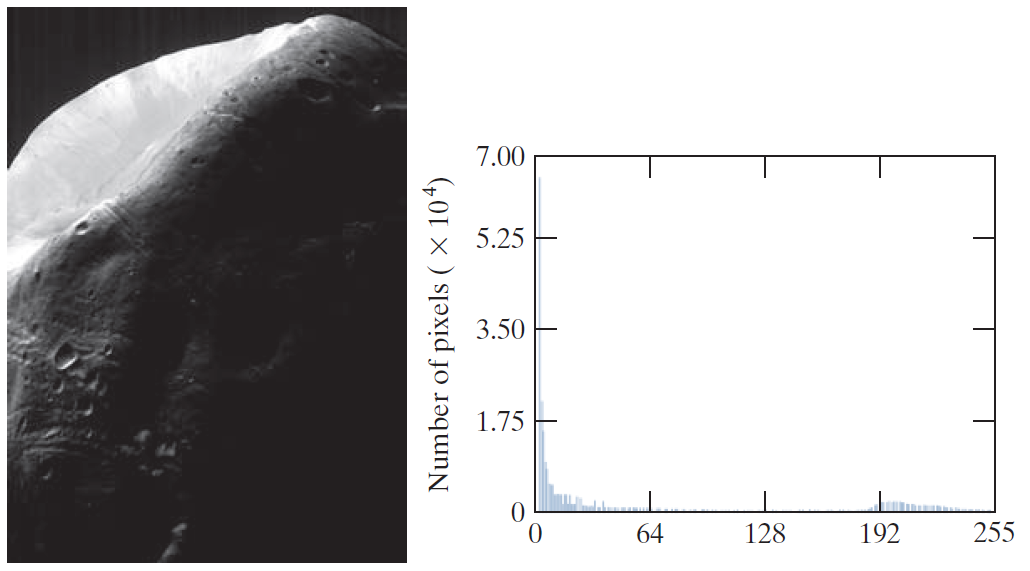
\includegraphics[width=\linewidth, height=6cm, keepaspectratio]{figuras/Fig_3_23.png}
            \caption{(a) An image, and (b) its histogram.}
    \end{figure}
\end{frame}

\begin{frame}{Resultado de la Ecualización de Histograma en Phobos}
    \begin{figure}
            % Reemplazar 'phobos_original.png' con el nombre de tu archivo de imagen
            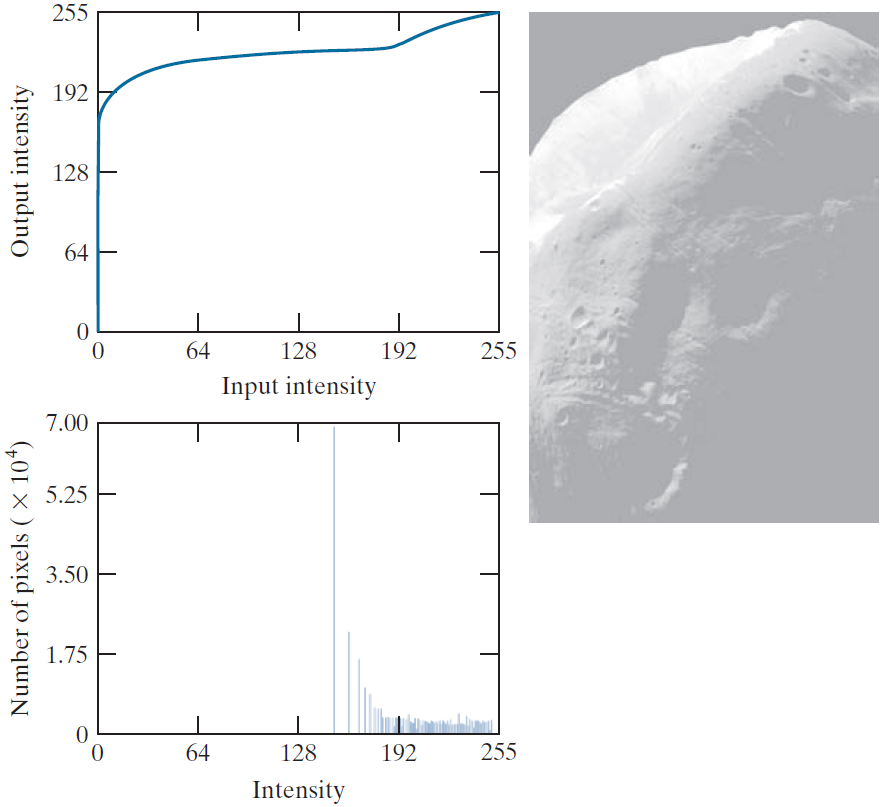
\includegraphics[width=0.4\linewidth]{figuras/Fig_3_24.png}
            \caption{\footnotesize{(a) Histogram equalization transformation obtained using the histogram in Fig. 3.23(b). (b) Histogram equalized image. (c) Histogram of equalized image.}}
    \end{figure}
    \begin{alertblock}{\footnotesize Problema}\footnotesize
        La ecualización mapea un intervalo estrecho de píxeles oscuros a la parte alta de la escala de grises. El resultado es una imagen con apariencia lavada y pérdida de detalle en las zonas originalmente oscuras.
    \end{alertblock}
\end{frame}

%------------------------------------------------
\section{Especificación de Histograma}
%------------------------------------------------

\begin{frame}{Especificación de Histograma: Fundamentos}\footnotesize
    \begin{block}{Objetivo}
        Modificar una imagen para que su histograma coincida (aproximadamente) con una forma específica deseada, en lugar de simplemente aplanarlo. Esto permite un control más fino sobre el realce.
    \end{block}
    \textbf{Proceso General:}
    \begin{enumerate}
        \item Obtener la transformación de ecualización de la imagen original: $s = T(r)$.
        \item Especificar la función de densidad de probabilidad deseada $p_z(z)$.
        \item Calcular la transformación $G(z)$ basada en $p_z(z)$:
              \begin{equation}
                  v_k = G(z_k) = (L-1) \sum_{j=0}^{k} p_z(z_j) \label{eq:hist_spec_G}
              \end{equation}
        \item Encontrar la transformación inversa $z_k = G^{-1}(s_k)$. Esto implica mapear los valores $s_k$ (obtenidos de la ecualización de la imagen original) a los valores $z_k$ usando la CDF del histograma especificado. Para cada $s_k$, se busca el $z_j$ tal que $G(z_j) \ge s_k$ (se elige el menor $j$).
        \item Aplicar $G^{-1}$ a la imagen ecualizada (o directamente componer transformaciones). Los valores $z_k$ son los nuevos niveles de gris.
    \end{enumerate}
\end{frame}

\begin{frame}{Aplicación a Phobos: Especificación}\footnotesize
    \begin{block}{\footnotesize Estrategia}
        Modificar el histograma original para que tenga una transición más suave en los niveles oscuros, preservando la forma general.
    \end{block}
    \begin{columns}[T]
        \begin{column}{0.3\textwidth}
            Fig. 3.25 Especificación del Histograma, a) Histograma especificado, b) Transformación $G(z_{q})$, etiquetada como (1), y $G^{-1}(s_{k})$, etiquetada como (2). c) Resultado de la especificación del histograma. b) Histograma de la imagen c)
        \end{column}
        \begin{column}{0.7\textwidth}
            \begin{figure}
                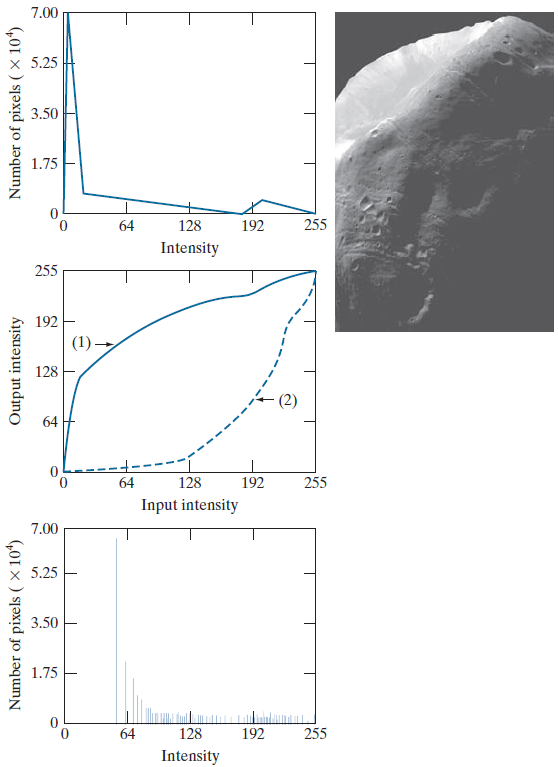
\includegraphics[width=0.5\linewidth]{figuras/Fig_3_25.png}
           \end{figure}
        \end{column}
    \end{columns}
\end{frame}

\begin{frame}{Resultado de la Especificación de Histograma en Phobos}
    \begin{block}{Mejora}
        La imagen resultante de la especificación de histograma muestra una mejora significativa en la apariencia y visibilidad de detalles en comparación con la ecualización directa. Un cambio modesto en el histograma objetivo fue suficiente.
    \end{block}
\end{frame}

%------------------------------------------------
\section{Resumen y Conclusiones}
%------------------------------------------------

\begin{frame}{Comparación y Conclusiones}\footnotesize
    \begin{block}{Ecualización de Histograma}
        \begin{itemize}
            \item \textbf{Ventaja:} Simple, automático, no requiere parámetros.
            \item \textbf{Desventaja:} Puede producir resultados no deseados (e.g., "lavado") si el histograma original tiene grandes picos, ya que busca un histograma plano que no siempre es ideal.
        \end{itemize}
    \end{block}
    \pause
    \begin{alertblock}{Especificación de Histograma}
        \begin{itemize}
            \item \textbf{Ventaja:} Ofrece mayor control sobre la forma del histograma de salida, permitiendo realces más adaptados al contenido de la imagen o a un objetivo visual particular.
            \item \textbf{Desventaja:} Requiere la definición de un histograma objetivo, lo cual puede no ser trivial y podría necesitar experimentación.
        \end{itemize}
    \end{alertblock}
    \pause
    \begin{exampleblock}{Lección del Ejemplo de Phobos}
        Para imágenes con distribuciones de intensidad muy sesgadas, la especificación de histograma es a menudo una mejor elección que la ecualización directa si se desea un realce más natural y detallado.
    \end{exampleblock}
\end{frame}


\begin{frame}[fragile]{Ejemplo 3.8 Comparison between histogram equalization and histogram specification}

\href{run:Ejemplo_3_8_p1.html}{CLICK AQUI}

\end{frame}



%%%%%%%%%%%%%%%%%%%%%%%%%%%%%%%%%%%%%%%%%%%%%%%%%%%%%%%%%%%%%%%%%%%%%%%%%%%%%%%%%%%%%%%%%%%%%%%%%%%%%%%%%%%%%%%%%%%%%%%%%%%%%%%%%%%%%%%%%%%%%%%%%%%%%%%%%%%%%%%%%%%%%%%%%%%%%%%%%%%%%%%%%%%%%%%%%%%%%%%%%%%%%%5


\title[Ejemplo]{Procesamiento del Histograma Local}
\subtitle{}
\author[Tu Nombre/Institución]{}
\date{}
\institute{}
% --- Diapositiva de título ---
\begin{frame}
  \titlepage
\end{frame}

%------------------------------------------------
\section{Procesamiento Local de Histogramas}
%------------------------------------------------
\begin{frame}{Limitaciones del Procesamiento Global}
    \begin{block}{Problema Principal}
        Los métodos globales (ecualización o especificación) modifican píxeles basados en el histograma de la \textbf{imagen completa}.
    \end{block}
    Esto es adecuado para un realce general, pero a menudo falla cuando el objetivo es:
    \begin{itemize}
        \item Realzar detalles en áreas pequeñas.
        \item Adaptarse a variaciones locales de iluminación o contraste.
    \end{itemize}
    La razón es que el número de píxeles en áreas pequeñas tiene una influencia insignificante en el cálculo de las transformaciones globales.
    \begin{alertblock}{Solución}
        Diseñar funciones de transformación basadas en la distribución de intensidad de \textbf{vecindades de píxeles}.
    \end{alertblock}
\end{frame}

\begin{frame}{Procesamiento Local de Histogramas: Metodología}\tiny
    \begin{block}{Procedimiento}
        Las técnicas de procesamiento de histograma (ecualización/especificación) pueden adaptarse para el realce local:
        \begin{enumerate}\footnotesize
            \item \textbf{Definir una vecindad:} Se elige una forma y tamaño para la vecindad (e.g., $3 \times 3$, $5 \times 5$ píxeles).
            \item \textbf{Desplazar la vecindad:} El centro de la vecindad se mueve de píxel a píxel a través de la imagen.
            \item \textbf{En cada ubicación:}
                \begin{itemize}\footnotesize
                    \item Se calcula el histograma de los píxeles \textbf{dentro de la vecindad actual}.
                    \item Se obtiene una función de transformación (ecualización o especificación) basada en este histograma local.
                    \item Esta función se usa para mapear la intensidad del \textbf{píxel central} de la vecindad.
                \end{itemize}
            \item \textbf{Repetir:} El proceso se repite para cada píxel de la imagen.
        \end{enumerate}
    \end{block}
    \begin{exampleblock}{Consideraciones Computacionales}
        \begin{itemize}
            \item \textbf{Actualización eficiente:} Al mover la vecindad un píxel, solo una fila/columna cambia. Es posible actualizar el histograma local incrementalmente en lugar de recalcularlo desde cero, ahorrando cómputo.
            \item \textbf{Regiones no solapadas:} Usar regiones que no se solapan reduce el cómputo, pero puede producir un "efecto de bloques" indeseable.
        \end{itemize}
    \end{exampleblock}
\end{frame}

\begin{frame}{Ejemplo 3.9: Ecualización Local de Histogramas}\tiny
    \begin{block}{\footnotesize Escenario del Ejemplo}
    Una imagen de 8 bits, $512 \times 512$, con cinco cuadrados negros sobre un fondo gris claro. La imagen es ligeramente ruidosa (imperceptible). Hay objetos incrustados en los cuadrados oscuros, invisibles en la imagen original.
    \end{block}

    \begin{figure}
            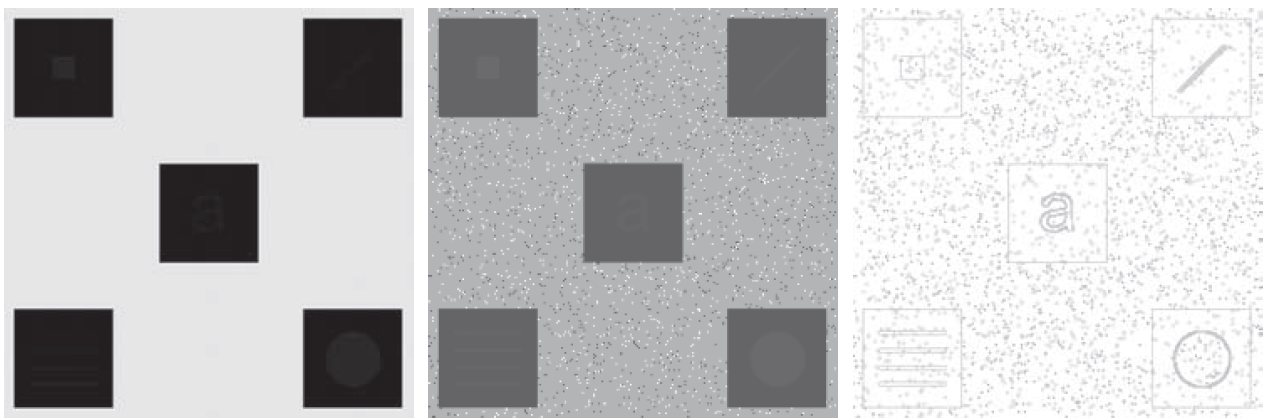
\includegraphics[width=0.8\linewidth]{figuras/Fig_3_26.png}
            \caption{\tiny (a) Objetos dentro de los cuadrados no son visibles. (b) Ruido realzado, pero sin revelar detalles significativos de los objetos. (c) Detalle significativo visible dentro de los cuadrados oscuros.}
    \end{figure}
    \begin{alertblock}{\tiny Observación Clave}
    La ecualización local (con vecindad $3 \times 3$) revela detalles significativos dentro de los cuadrados oscuros. Los valores de intensidad de estos objetos son demasiado cercanos a los de los cuadrados y sus tamaños demasiado pequeños para influir significativamente en la ecualización global.
    \end{alertblock}
\end{frame}

%------------------------------------------------
\section{Resumen y Conclusiones}
%------------------------------------------------

\begin{frame}{Comparación y Conclusiones}\tiny
    \begin{block}{Ecualización de Histograma Global}
        \begin{itemize}
            \item \textbf{Ventaja:} Simple, automático.
            \item \textbf{Desventaja:} Puede producir "lavado" si hay picos grandes; no siempre ideal. Falla en realzar detalles en áreas pequeñas si no son estadísticamente significativas globalmente.
        \end{itemize}
    \end{block}
    \pause
    \begin{alertblock}{Especificación de Histograma Global}
        \begin{itemize}
            \item \textbf{Ventaja:} Mayor control sobre la forma del histograma de salida.
            \item \textbf{Desventaja:} Requiere definir un histograma objetivo. También sufre de las limitaciones globales para detalles locales.
        \end{itemize}
    \end{alertblock}
    \pause
    \begin{exampleblock}{Procesamiento Local de Histogramas}
        \begin{itemize}
            \item \textbf{Ventaja:} Efectivo para realzar detalles en áreas pequeñas y adaptarse a condiciones locales. Revela información no visible con métodos globales.
            \item \textbf{Desventaja:} Computacionalmente más intensivo. Puede realzar ruido. La elección del tamaño de la vecindad es crucial.
        \end{itemize}
    \end{exampleblock}
     \begin{block}{Lección General}
        La elección entre métodos globales y locales (y entre ecualización y especificación) depende del contenido de la imagen y de los objetivos específicos del realce. Para detalles finos en regiones localizadas, el procesamiento local es superior.
    \end{block}
\end{frame}

%%%%%%%%%%%%%%%%%%%%%%%%%%%%%%%%%%%%%%%%%%%%%%%%%%%%%%%%%%%%%%%%%%%%%%%%%%%%%%%%%%%%%%%%%%%%%%%%%%%%%%%%%%%%%%%%%%%%%%%%%%%%%%%%%%%%%%%%%%%%%%%%%%%%%%%%%%%%%%%%%%%%%%%%%%%%%%%%%%%%%%%%%%%%%%%%%%%%%%%%%%%%%%%%%


\begin{frame}[fragile]{UTILIZANDO LA ESTADÍSTICA DEL HISTOGRAMA PARA MEJORAR LA IMAGEN}

\href{run:Tema_pag_150_p1.html}{CLICK AQUI}

\end{frame}


\begin{frame}[fragile]{3.4 FUNDAMENTOS DEL FILTRADO ESPACIAL}

\href{run:Tema_3_4_p1.html}{OBJETIVO 3.4 CLICK AQUI}

\end{frame}

\begin{frame}[fragile]{CORRELACIÓN ESPACIAL Y CONVOLUCIÓN}

\href{run:Tema_3_4_pag_154_p1.html}{CORRELACIÓN Y CONVOLUCIÓN ESPACIAL CLICK AQUI}

\end{frame}

\begin{frame}[fragile]{NÚCLEOS SEPARABLES DE FILTROS}

\href{run:Tema_3_4_pag_161_p1.html}{NÚCLEOS SEPARABLES DE FILTROS}

\end{frame}


\begin{frame}[fragile]{LOWPASS GAUSSIAN FILTER KERNELS}

\href{run:Tema_3_4_pag_166_p1.html}{LOWPASS GAUSSIAN FILTER KERNELS}

\end{frame}

\begin{frame}[fragile]{Ejemplos: LOWPASS GAUSSIAN FILTER KERNELS}

\href{run:Tema_3_4_pag_169_p1.html}{Ejemplos: LOWPASS GAUSSIAN FILTER KERNELS}

\end{frame}

\begin{frame}[fragile]{FILTROS DE ESTADÍSTICA DE ORDEN}

\href{run:Tema_3_4_pag_174_p1.html}{FILTROS DE ESTADÍSTICA DE ORDEN}

\end{frame}

\begin{frame}[fragile]{FILTROS ESPACIALES DE REALCE (PASA ALTAS)}

\href{run:Tema_3_6_p1.html}{3.6 FILTROS ESPACIALES DE REALCE (PASA ALTAS)}

\end{frame}

\begin{frame}[fragile]{Enmascaramiento desenfocado y filtrado high-boost}

\href{run:Tema_3_6_pag_182.html}{Enmascaramiento desenfocado y filtrado high-boost}

\end{frame}

\begin{frame}[fragile]{Derivadas de Primer Orden para Realce de Imágenes: El Gradiente}

\href{run:Tema_3_6_pag_184.html}{Derivadas de Primer Orden para Realce de Imágenes: El Gradiente}

\end{frame}

\begin{frame}[fragile]{Filtros de Señal: Highpass, Bandreject y Bandpass derivados de Lowpass}

\href{run:Tema_3_7_pag_188.html}{3.7 Filtros de Señal: Highpass, Bandreject y Bandpass derivados de Lowpass}

\end{frame}

\begin{frame}[fragile]{Métodos de Mejora Espacial en Procesamiento de Imágenes}

\href{run:Tema_3_8_pag_191.html}{3.8 Métodos de Mejora Espacial en Procesamiento de Imágenes}

\end{frame}


% ANTES: \href{run:Tema_3_8_pag_191.html}{...}
% DESPUÉS (EJEMPLO):
\href{run:Tema_3_8_pag_191.html}{3.8 Métodos de Mejora Espacial en Procesamiento de Imágenes}

\begin{frame}[fragile]{Métodos de Mejora Espacial en Procesamiento de Imágenes}

% Reemplaza "https://tudominio.com/Presentation/Tema_3_8_pag_191.html" con la URL real y completa del archivo.
\href{https://1drv.ms/u/s!AmnSq06Ge2Zqks5zTf2hhng2VKFo2w?e=SAB90N}{3.8 Métodos de Mejora Espacial en Procesamiento de Imágenes}

\end{frame}




\end{document}
